% !TEX encoding = UTF-8 Unicode
% !TEX root = thesis-ex.tex

\section{The Large Hadron Collider}
The Large Hadron Collider (LHC) is a part of the European Organization for Nuclear Research (CERN).
It has a circumference of 27 kilometers, making it the world's largest particle accelerator, and is housed in a tunnel that is up to 175 meters below the surface of the earth.
The LHC ring has eight arcs and eight straight sections, with each straight section being approximately 528 m long.
Four of the straight sections are where the major detectors are located, while the other four are used for machine utilities, radio frequency, collimation and beam dumps.
The arc sections are built using 1232 dipole superconducting magnets, providing a magnetic field of up to 8.33 T.
Another 392 quadrupole magnets are used for focussing the particle beam.
Sixteen radio frequency (RF) cavities that provide a voltage of 2 MV and operate at 400 MHz are used to accelerate the proton or ion beams that are kept in their circular path by the dipole magnets.
The magnets are cooled down to 1.9 K via liquid Helium.

The LHC beam pipe has two rings with the counter-rotating beams and uses a uses a twin-bore magnet design that optimizes for both cost, as well as space.
The counterrotating beams require opposite magnetic dipole fields in both rings, with separate magnetic and vacuum chambers, with the common sections only at the insertion regions and where the major experimental detectors are located.
These detectors are: A Toroidal LHC Apparatus (ATLAS), Compact Muon Solenoid (CMS), A Large Ion Collider Experiment (ALICE), and Large Hadron Collider - Beauty (LHCb) \cite{Evans:2008zzb}.

Studying the rare events that the LHC was designed for requires high beam energies and intensities, and the LHC is capable of reaching up to center of mass energies, \sqrts\ = 14 TeV for protons and \sqrtsnn\ = 5.5 TeV for lead ions.
The LHC delivers up to $10^{34} \mathrm{cm}^2\mathrm{s}^1$ of luminosity to the ATLAS and CMS detectors when colliding protons.
The LHCb detector is a lower luminosity experiment, that receives up to $10^{32} \mathrm{cm}^2\mathrm{s}^1$, and ALICE, a dedicated ion experiment aims at a peak luminosity of $10^{27} \mathrm{cm}^2\mathrm{s}^1$ for nominal lead-lead operation.
In 2015, the LHC delivered an integrated luminosity of 0.49 \pb\ of \pbpb\ and 25 \pb\ of \pp\ data.

A schematic of the entire accelerator complex and the path followed by protons and heavy ions is show in Figure~\ref{fig:cern}.
The protons in the LHC are obtained by stripping a hydrogen atom of its electrons with an electric field.
They are then supplied to the LHC via the Linac2 - Proton Synchrotron Booster - Proton Synchrotron - Super Proton Synchrotron chain.
The complete ionization of lead on the other hand is done in multiple stages, with the first stage in Linac3, which provides $\mathrm{Pb}^{+29}$ via an ion source.
The $\mathrm{Pb}^{+29}$ lead ions are further stripped of electrons by passing them through a 0.3 $\mu$m foil.
The $\mathrm{Pb}^{+54}$ ions are selected via mass spectrometer and sent to the Low Energy Ion Ring (LEIR), followed by the Proton Synchrotron and Super Proton Synchrotron, and then finally the LHC.
The final stripping of lead ions takes place after the PS, on a 0.8 mm thin aluminum foil.


\begin{figure}[ht]
	\centering
	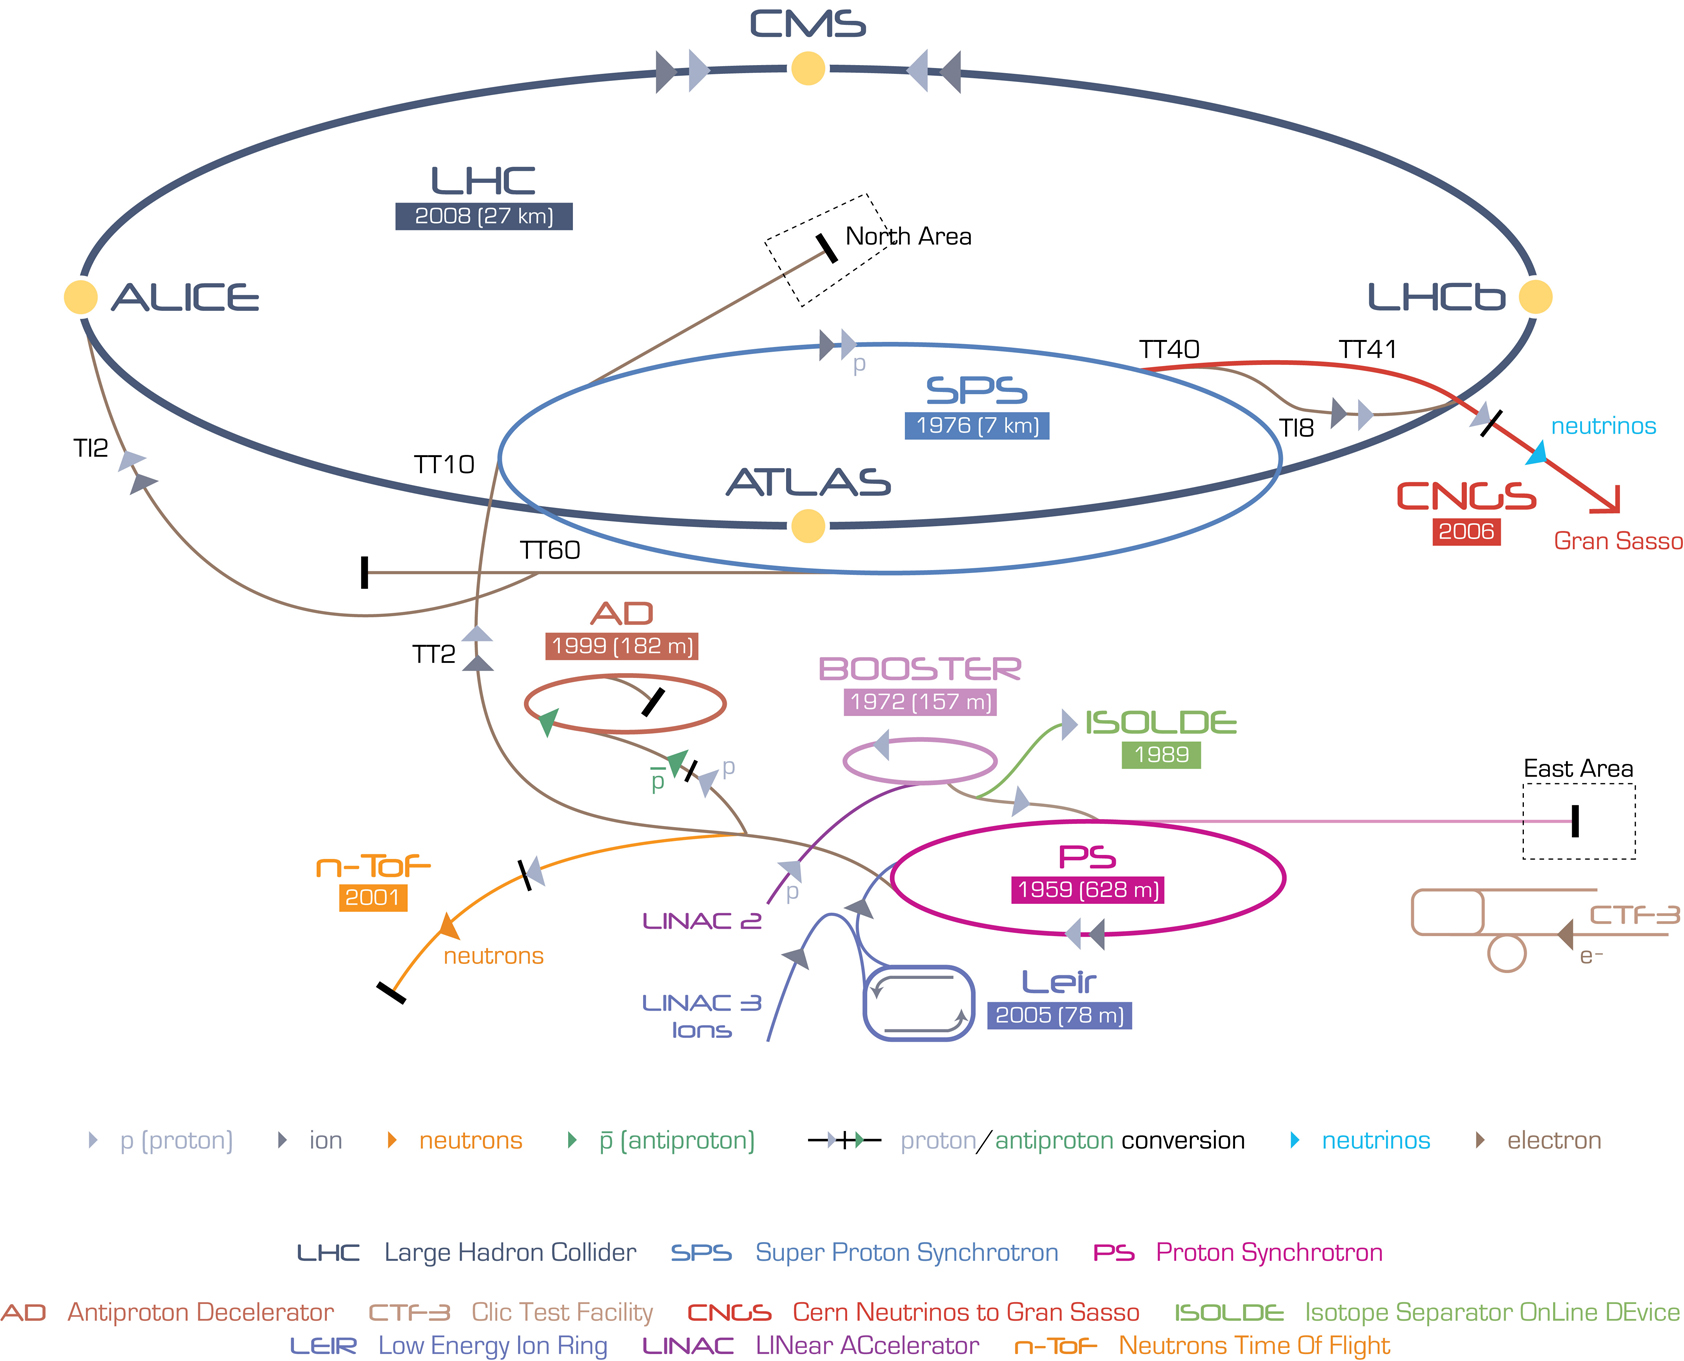
\includegraphics[width=0.8\textwidth]{figures/setup/cern.jpg} %
	\caption{The accelerator complex at CERN.
ATLAS can be seen inside the SPS on the LHC ring.
Figure from Ref.~\cite{Christiane:1260465}.}
	\label{fig:cern}%
\end{figure}

%The LHC beams have a nominal bunch spacing of 25 ns corresponding to 2808 bunches for \pp\ and a bunch spacing of 100 ns corresponding to 492 bunches for \pbpb.

\section{The ATLAS Detector}
The ATLAS detector (Figure~\ref{fig:atlas}) is a general purpose detector at the LHC.
It uses a right-handed coordinate system with its origin at the nominal interaction point (IP) in the
 centre of the detector and the $z$-axis along the beam pipe.
The $x$-axis points from the IP to the centre of the LHC ring, and the $y$ axis points upward.
Cylindrical coordinates 
 $(r,\phi)$ are used in the transverse plane, $\phi$ being the azimuthal angle around the beam pipe.
The pseudorapidity is defined in terms of the polar angle $\theta$ as 
 $\eta=-\ln\tan(\theta/2)$.
The detector is symmetric in the forward-backward direction, with the positive $z$ direction being the $A$ side, and the negative $z$ direction being the $C$ side.
It has full $2\pi$ coverage in azimuth.
 The transverse momentum \pt, the transverse energy \Et, and the missing transverse energy \Etmiss\ are defined in the $x-y$ plane unless stated otherwise.
The distance $\Delta R$ in the pseudorapidity-azimuthal angle space is defined as $\Delta R = \sqrt{\Delta \eta^2 + \Delta \phi^2}$.

The detector was designed keeping in mind the goals of the physics it aimed to explore, and as such has the following characteristics:
\begin{itemize}
\item Fast, radiation-hard electronics and sensor
\item Fine granularity to be able to manage large particle fluxes
\item Large acceptance in pseudorapidity and full azimuthal coverage
\item Good electromagnetic calorimetry for photon and electron identification
\item Good hadron calorimetry for accurate jet and missing transverse energy measurements
\item Good muon identification and momentum resolution
\item Highly efficient trigger system 
\end{itemize}

\begin{figure}[ht]
	\centering
	\includegraphics[width=0.7\textwidth]{figures/setup/atlas.pdf}
	\caption{The ATLAS detector.
Figure from Ref.~\cite{Aad:2008zzm}.}	
	\label{fig:atlas}
\end{figure}


These design goals are achieved with the main subsystems: the inner detector, the calorimeter, the muon spectrometer, and the trigger system.
The main analysis discussed in this thesis uses the inner detector, calorimeter, and the trigger system.
The muon system is described for completeness.


\subsection{Inner Detector}
The inner detector shown in Figure.~\ref{fig:inner_det} is designed to reconstruct the charged particle trajectories for particles with momenta down to 0.5 GeV in the interval $|\eta| < 2.5$.
It is immersed in a 2T magnetic field from the central solenoid that covers a region of 5.3 m long and has a diameter of 2.5 m.
The inner detector has capabilities for pattern recognition, momentum and vertex measurements, and electron identification.
These measurements are made using the inner pixel detector, the semi-conductor tracker (SCT), and the transition radiation tracker (TRT).


\subparagraph{Pixel system: } This system is segmented in \rphi and comprises of four pixel layers : the innermost insertable B layer (IBL) and three identical silicon pixel detectors.
The IBL was added to the ATLAS detector during the first long shutdown of the LHC in 2013-2014.
It consists of 14 carbon fiber staves, 2 cm wide and 64 cm long, surrounding the beam pipe at a mean radius of 33 mm, and covering a pseudorapidity region of $\pm 3$.
Each stave consists of 26880 pixels in a matrix of 80 columns (50 $\mu$m pitch), by 336 rows (250 $\mu$m pitch) \cite{LaRosa:2016nbd, Capeans:1291633}.
The other three layers layers have a pixel size in $\rphi \times z$ of $50 \times 400 \mu \mathrm{m}^2$.
The accuracies in the barrel region are $10 \mu \mathrm{m}^2$ (\rphi) and $115 \mu \mathrm{m}^2 (z)$.
The end cap regions have an accuracy of $10 \mu \mathrm{m}^2 (\rphi) $ and $115 \mu \mathrm{m}^2 (R)$.
The hit resolution ranges from $\sim$8 (\rphi) and $\sim$40$\mu$m) ($z$) for the innermost layer, to $\sim$10 $\mu$m (\rphi) and $\sim$115$\mu$m ($z$) for the next three layers \cite{Aad:2008zzm}.
The pixel detector has approximately 80.4 million readout channels.


\subparagraph{Semi Conductor Tracker:} This subsystem has a coverage that overlaps with the pixel layers, and is arranged in concentric cylinders around the beam axis, with the end caps being disks perpendicular to the beam axis.
The SCT has eight strip (80 $\mu$m pitch) layers that are crossed by each track.
Small angle stereo strips (40 mrad) are used to measure both coordinates, with one set of strips in each layer, parallel to the beam direction.
The end cap region has nine layers of double sided modules with strips in the radial direction, with each also having a mean pitch of 80 $\mu$m.
The intrinsic resolution is $\sim$17$\mu$m (\rphi) and $\sim$580$\mu$m ($z$).
There are approximately 6.3 million readout channels from the SCT \cite{Aad:2008zzm}.


\subparagraph{Transition Radiation Tracker:} The TRT uses a combination of a xenon based gas and 4mm diameter straw tubes and provides for a large number of hits (up to 36) per track.
It covers the region $|\eta| <  2.0$, and has a resolution of $\sim$130$\mu$m in $r-\phi$, with no information in the $z$ direction.
The barrel region of the TRT has straws that are 144 cm long and are parallel to the beam axis, with the wires divided into two halves at $\eta = 0$.
The end-caps have 37 cm long straws in a radial configuration.
The TRT has approximately 315,000 channels \cite{Aad:2008zzm}.


\begin{figure}[ht]
	\centering
        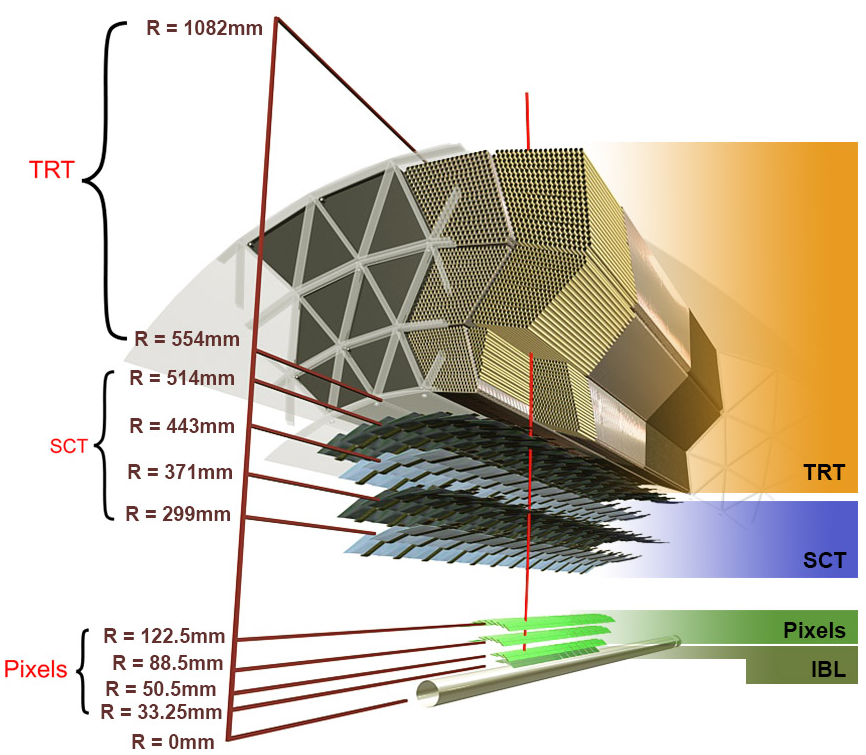
\includegraphics[width=0.7\textwidth]{figures/setup/inner_det.png}
          \caption{ATLAS Inner Detector System.
          Figure from Ref.~\cite{Potamianos:2209070}.}
          \label{fig:inner_det}
\end{figure}

%%%%%%%%%%%%%%%%%%%%%%%%%%%%%%%%%%
\subsection{Calorimeter}
The calorimeter covers the range of $|\eta| < 4.9$ for using a variety of different techniques.
The parameters are summarized in the table below.
Over  $|\eta| < 2.5$, where there is overlap with the inner detector, the highly granular electromagnetic calorimeter is used for precision measurements of electrons and photons.
The rest of calorimeter has coarser granularity that is sufficient for jet reconstruction.
The calorimeter contains the electromagnetic and hadronic showers, and limits the punch through to the muon system.
The EMCal has a radiation depth greater than 22 radiation lengths in the barrel, and greater than 24 radiation lengths in the end caps.
The approximately 10 interaction lengths in the barrel and end cap provide good resolution for high energy jets.
The total thickness of the calorimeter is 11 interaction lengths at $\eta = 0$.
The calorimeter is divided into different subsystems, including the Liquid Argon Electromagnetic Calorimeter (LAr EMCal) and the Hadronic calorimeter (HCal).

\subparagraph{LAr EMCal: }
The EMCal covers the region $|\eta| < 1.475$ and has two end caps ($1.375 < |\eta| < 3.2$).
It also contains the central solenoid.
The barrel calorimeter is divided into two half barrels, separated by 4mm at $z = 0$.
Each end cap is divided into two coaxial wheels, with the inner one covering $2.5 < |\eta| < 3.2$ and the outer one covering  $1.375 < |\eta| < 2.5$.
The EMCal uses accordion shaped kapton electrodes and lead absorber plates that provide full azimuthal symmetry.
The EMCal is subdivided into three sections in its depth over $|\eta| < 2.5$, the region used for precision physics.
The $|\eta| < 1.8$ region also uses a pre-sampler detector that uses an active LAr layer to correct for energy lost upstream of the calorimeter.
A main source of this loss is the central solenoid.

\subparagraph{Hadronic Calorimeter: }
The hadronic calorimeter consists of the tile, LAr Hadronic end cap, and the LAr forward calorimeter.
The tile covers the region $|\eta| < 1.0$ , with its two barrels covering the range eta $0.8 < |\eta| < 1.7$.
It uses steel as the absorber and scintillating tiles for the active material.
The tile calorimeter extends radially from an inner radius of 2.28 m to 4.25 m.
It has a three layer that are 1.5, 4.1, and 1.8 interaction lengths thick in the barrel region, and 1.5, 2.6, and 3.3 interaction lengths in the extended barrel region.
The total detector thickness is 9.7 interaction lengths at $\eta = 0$.

The LAr hadronic end cap calorimeter (HEC) consists of two independent wheels per end cap, and is behind the EMCal end cap.
It extends out from $1.5 < |\eta| < 3.2$, and overlaps with the forward calorimeter and the tile calorimeter.
The HEC covers the radial region of 0.475 to 2.03 m.

The LAr Forward calorimeter (FCal) provides coverage over the $3.1 < |\eta| < 4.9$.
It is approximately 10 interaction lengths deep, and has three modules, one of which is optimized for electromagnetic measurements, while the other two for hadronic measurements.
Each module is made of concentric rods and tubes parallel to the beam axis.

A summary of the depth of the calorimeter in terms of the interaction lengths, as a function of pseudorapidity is shown in Figure~\ref{fig:interaction_lenghts}.

\begin{figure}[ht]
	\centering
        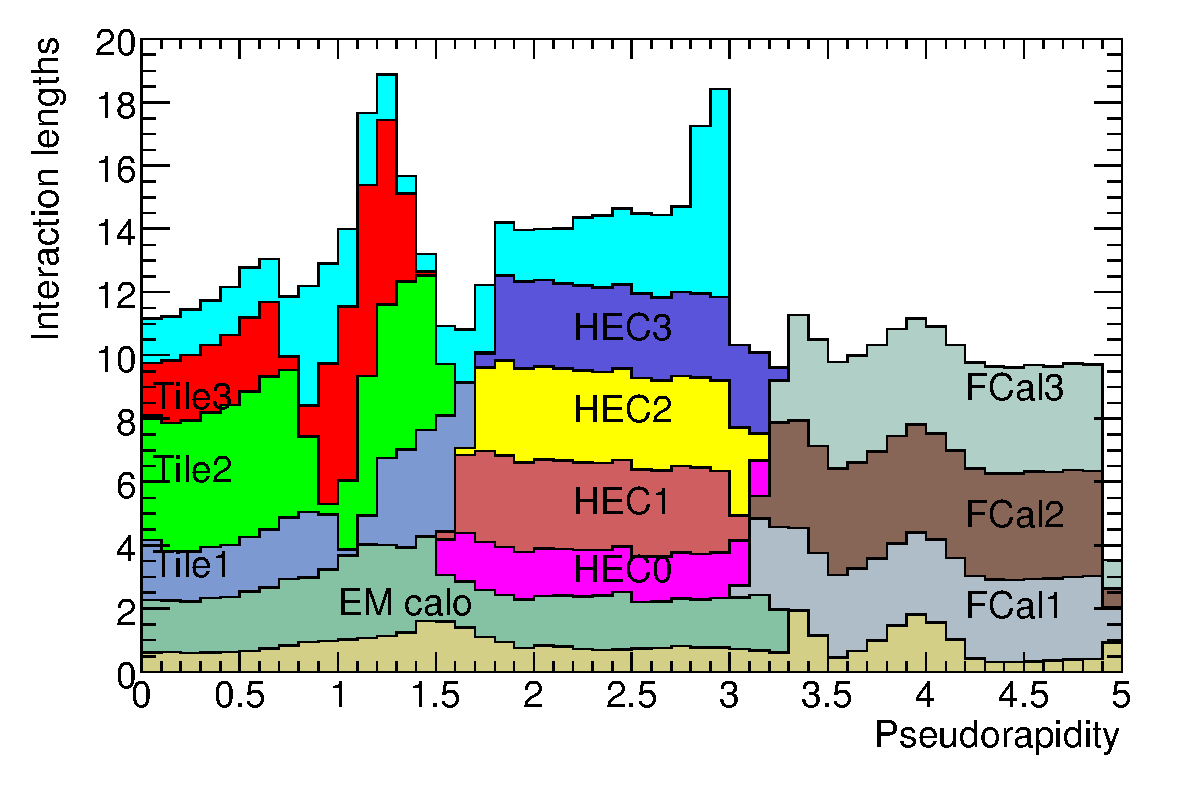
\includegraphics[width=0.7\textwidth]{figures/setup/interaction_lengths}
          \caption{Cumulative material in the calorimeter system in units of hadronic interaction length as a function of $|\eta|$.
          Figure from Ref.~\cite{Aad:2008zzm}.}
          \label{fig:interaction_lenghts}
\end{figure}


%%%%%%%%%%%%%%%%%%%%%%%%%%%%%%%%%%
\subsection{Muon Spectrometer}
The muon spectrometer is based on the magnetic deflection of muon tracks in the toroid magnets.
The barrel toroid provides bending over the $|\eta| < 1.4$ range, and the end cap magnets provide bending in the $1.6 < |\eta < 2.7$ range.
In the transition region ($1.4 < |\eta| < 1.6$), the magnetic deflection is from a combination of the barrel and end-cap fields.
The barrel region has tracks that are measured in chambers in a cylindrical configuration around the beam axis.
The transition and end-cap have chambers perpendicular to the beam axis.



%%%%%%%%%%%%%%%%%%%%%%%%%%%%%%%%%%
\subsection{Other subsystems}
Other major subsystems of the ATLAS detector include the Zero Degree Calorimeter (ZDC), the trigger system

\subparagraph{ZDC: }
The zero degree calorimeter plays a key role in determining the centrality of heavy ion collisions.
It consists of quartz rods and tungsten plates, and measures neutral particles at $|\eta| >= 8.2$.
It is made of four modules, one electromagnetic, and three hadronic.
The Modules are made of 11 tungsten plates that are perpendicular to the beam direction.
Photomultiplier tubes are used to detect the Cherenkov radiation from particle showers.


\subparagraph{Trigger System: }
The trigger and data acquisition system (TDAQ) have different subsystems that are associated with sub-detectors.
There are three distinct levels: L1, L2, and the event filter.
The latter two form the High Level Trigger (HLT) system.
The L1 trigger uses custom electronics, while the HLT is software based.
%The L1 trigger, shown in Figure~\ref{fig:L1_trigger}, uses custom electronics, while the HLT, shown in Figure~\ref{fig:HLT_trigger}, is software based.
Each level uses information from the previous level to select events.
%
%\begin{figure}[ht]
%	\centering
%        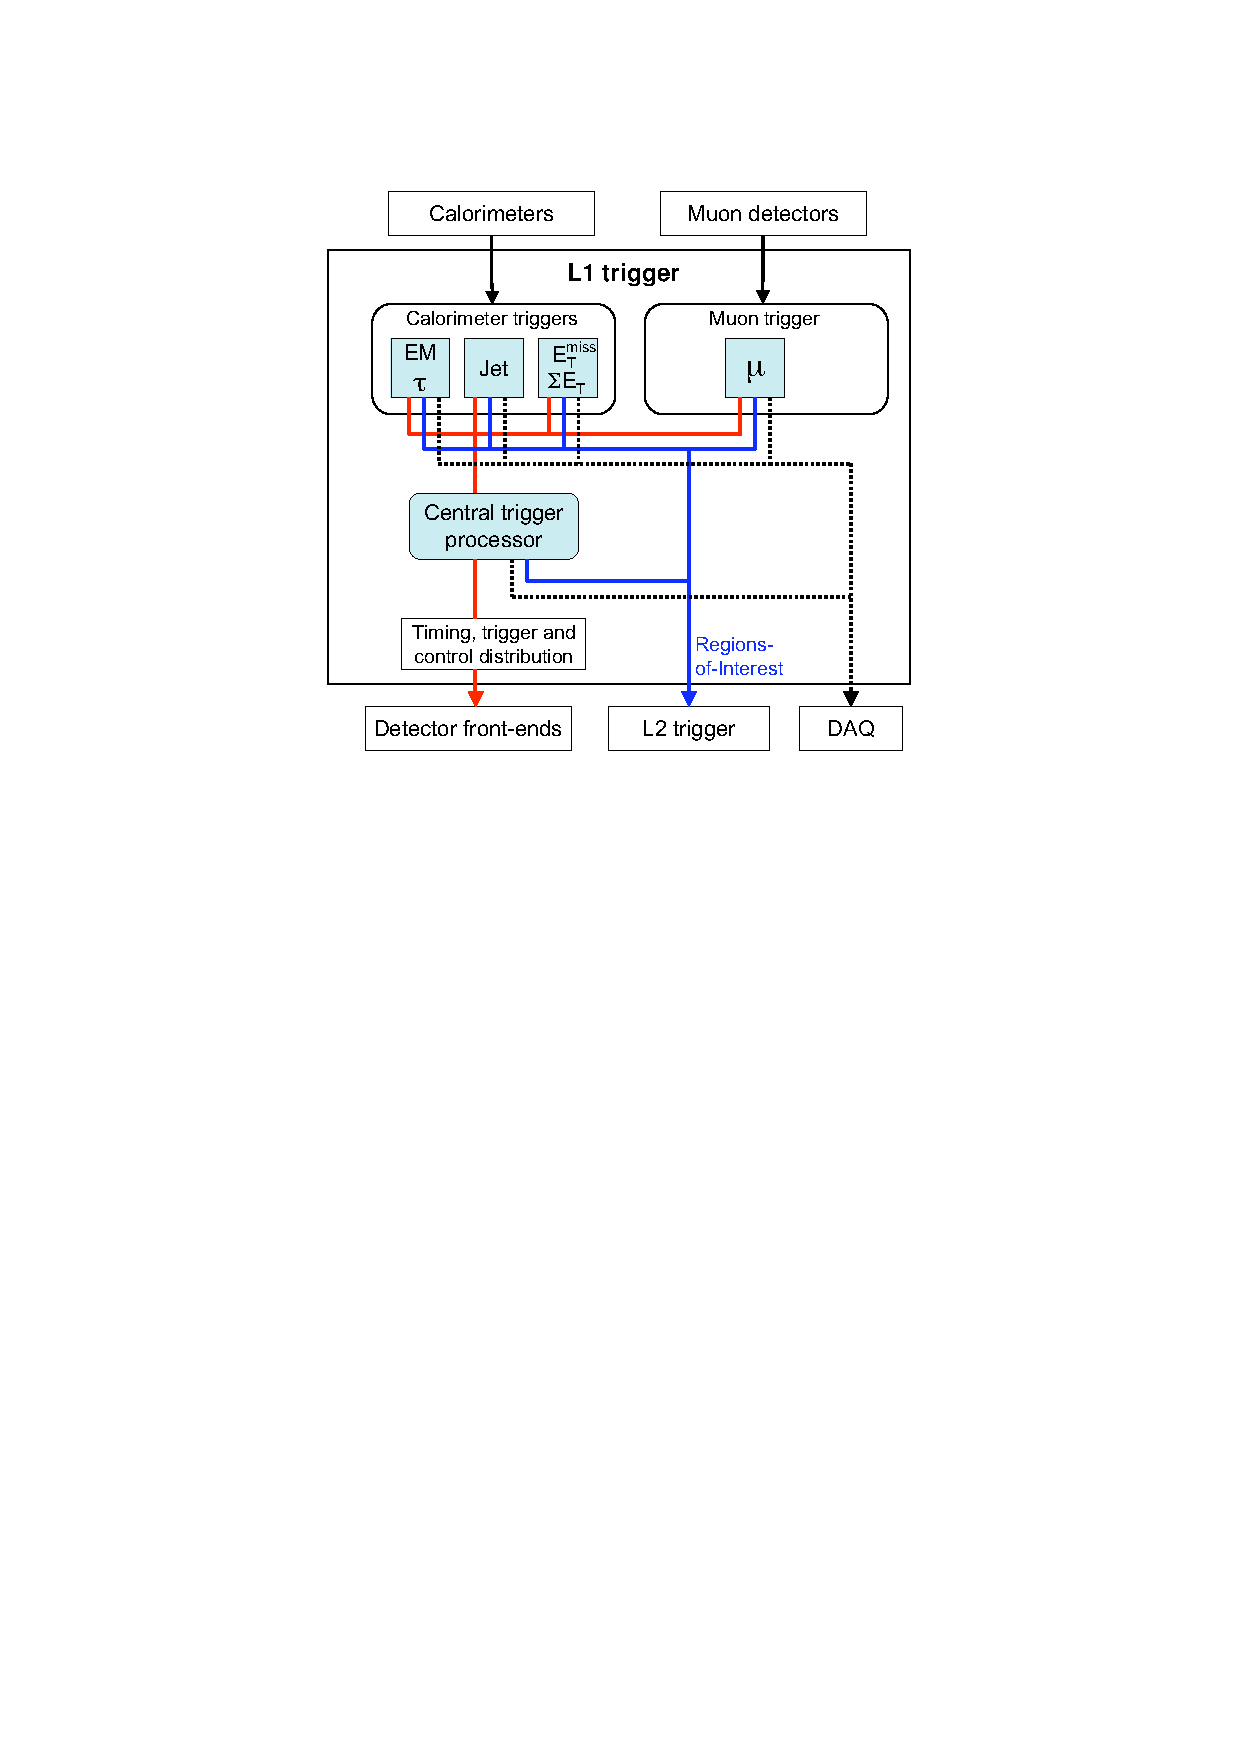
\includegraphics[width=0.7\textwidth]{figures/setup/L1_Trigger}
%          \caption{Block diagram of the L1 Trigger System.
%          Figure taken from Ref.~\cite{Aad:2008zzm}.}}
%          \label{fig:L1_trigger}
%\end{figure}
%
%\begin{figure}[ht]
%	\centering
%        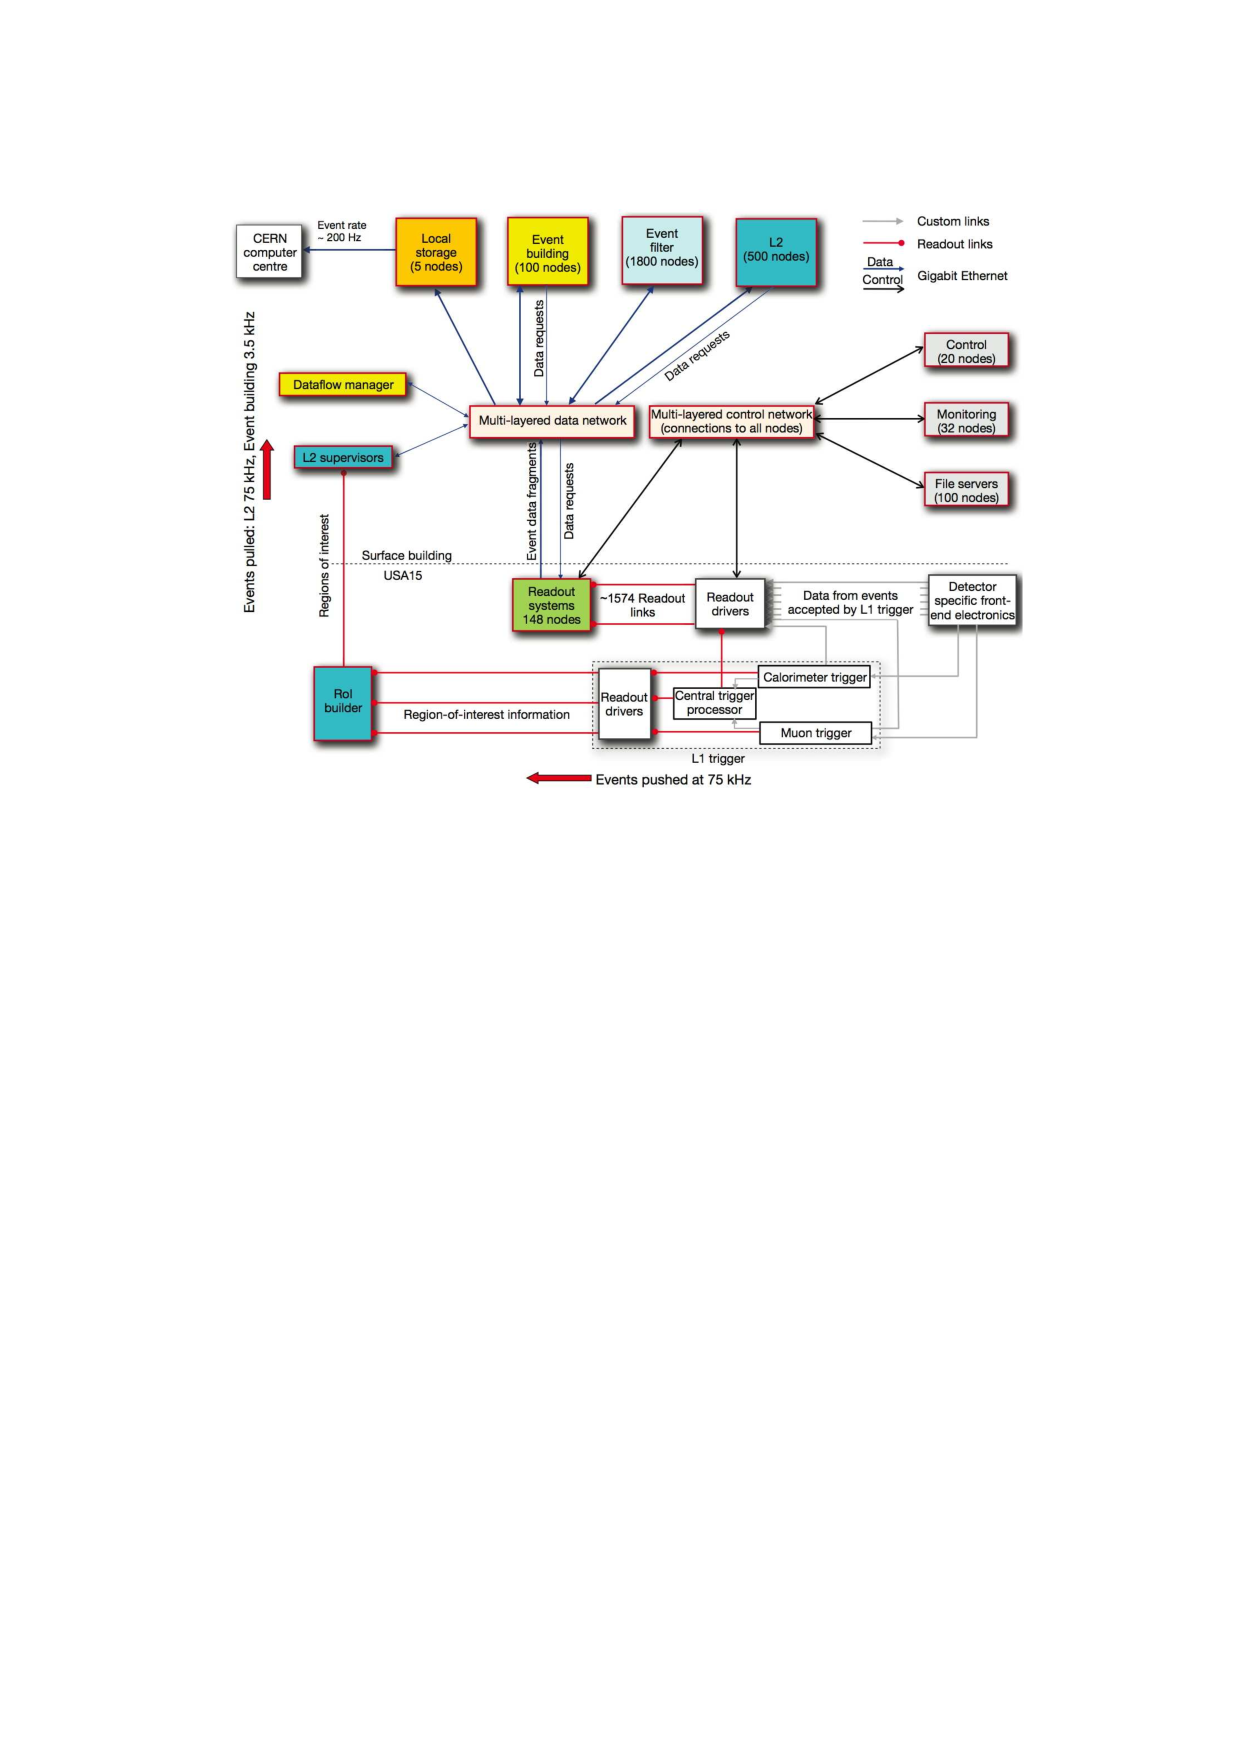
\includegraphics[width=0.7\textwidth]{figures/setup/HLT_Trigger}
%          \caption{Block diagram of the HLT Trigger system.
%          Figure taken from Ref.~\cite{Aad:2008zzm}.}
%          \label{fig:HLT_trigger}
%\end{figure}
The first level uses limited detector information and makes decisions based on muons, electron, photons, jets, and $\tau$-leptons carrying a high transverse momentum.
It is also capable of identifying large missing and total transverse energy.
 It has a maximum acceptance rate of 75kHz and makes a decision in less that 2.5$\mu$s.
This event rate is further reduced to 200 Hz by the HLT that uses the full granularity and precision of the inner detector, calorimeter and muon systems to select events.


%The $\eta$ coverage of the different detector systems can be seen in Figure~\ref{fig:atlaspseudorap}.
%\begin{figure}[htbp!]
%	\centering
%	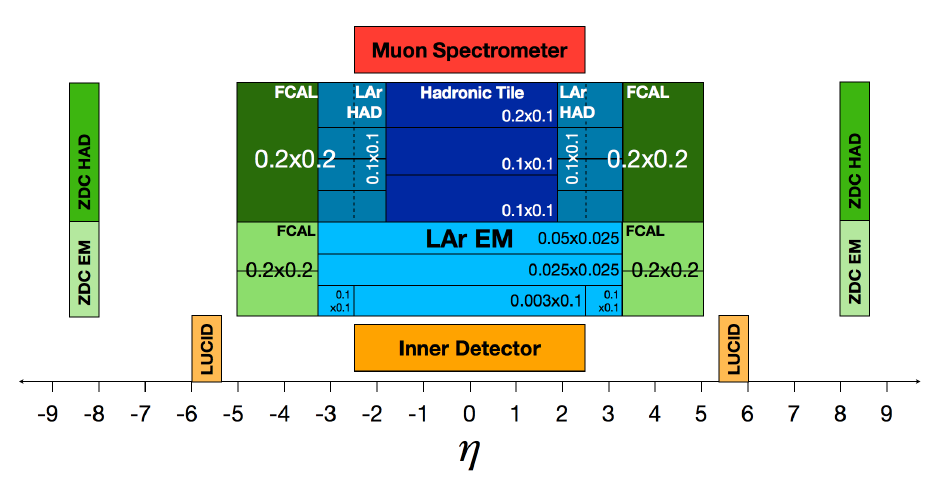
\includegraphics[width=0.7\textwidth]{figures/setup/atlaspseudorap.png} %
%	\caption{$\eta$ acceptance of the ATLAS detector.}	
%	\label{fig:atlaspseudorap}%
%\end{figure}

%%\begin{figure}[ht]
%%	\centering
%%	\includegraphics[width=0.7\textwidth]{figures/atlas.pdf} %
%%	\caption{The ATLAS detector.
%Figure taken from Ref.~\cite{Aad:2008zzm}.}	
%%	\label{fig:atlas}%
%%\end{figure}
%
%\subsection{Magnet System}
%The ATLAS detector has a magnet configuration that consists of a thin superconducting solenoid surrounding the inner detector cavity, and three large superconducting toroids arranged symmetrically around the calorimeters.
%The inner detector is immersed in a 2 T magnetic field, and achieves pattern recognition, momentum and vertex measurements, and electron identification by a combination of high resolution semiconductor pixel and strip detectors in the inner tracking volume, and a straw tube detector for transition radiation in the outer volume.

%\FloatBarrier


\section{Pileup and Centrality in ATLAS}
\label{sec:centrality}
% !TEX encoding = UTF-8 Unicode
% !TEX root = thesis-ex.tex
The FCal is a critical component in estimating the centrality of an event (See Section~\ref{sec:HICollisions} for an introduction to centrality).
While the direct measurement of the impact parameter is not possible, the centrality of an event directly correlates to number of reconstructed charged particles and the the energy deposited in the detector as shown in Figure~\ref{fig:nch_fcal}.
Thus, the energy deposited in the calorimeter can be used to estimate the centrality.
However, to avoid autocorrelations in the measurement, different detector regions are used for the analysis and the event classification.
Since the energy in the barrel region is directly correlated to the energy in the forward calorimeter as shown in Figure~\ref{fig:fcal_barrel}, event centrality can be determined using the transverse energy in the FCal, \ETfcal\.
The \ETfcal\. is divided in percentiles as shown in Figure~\ref{fig:fcal_distr}, with each bin corresponding to a centrality interval.
The 0--10\% centrality corresponds to most central collisions with the maximum overlap between the colliding nuclei, while the 90--100\% corresponds to the most peripheral collisions with the least overlap between the colliding nuclei.


 \begin{figure}
\centering
\begin{subfigure}{.45\textwidth}
  \centering
  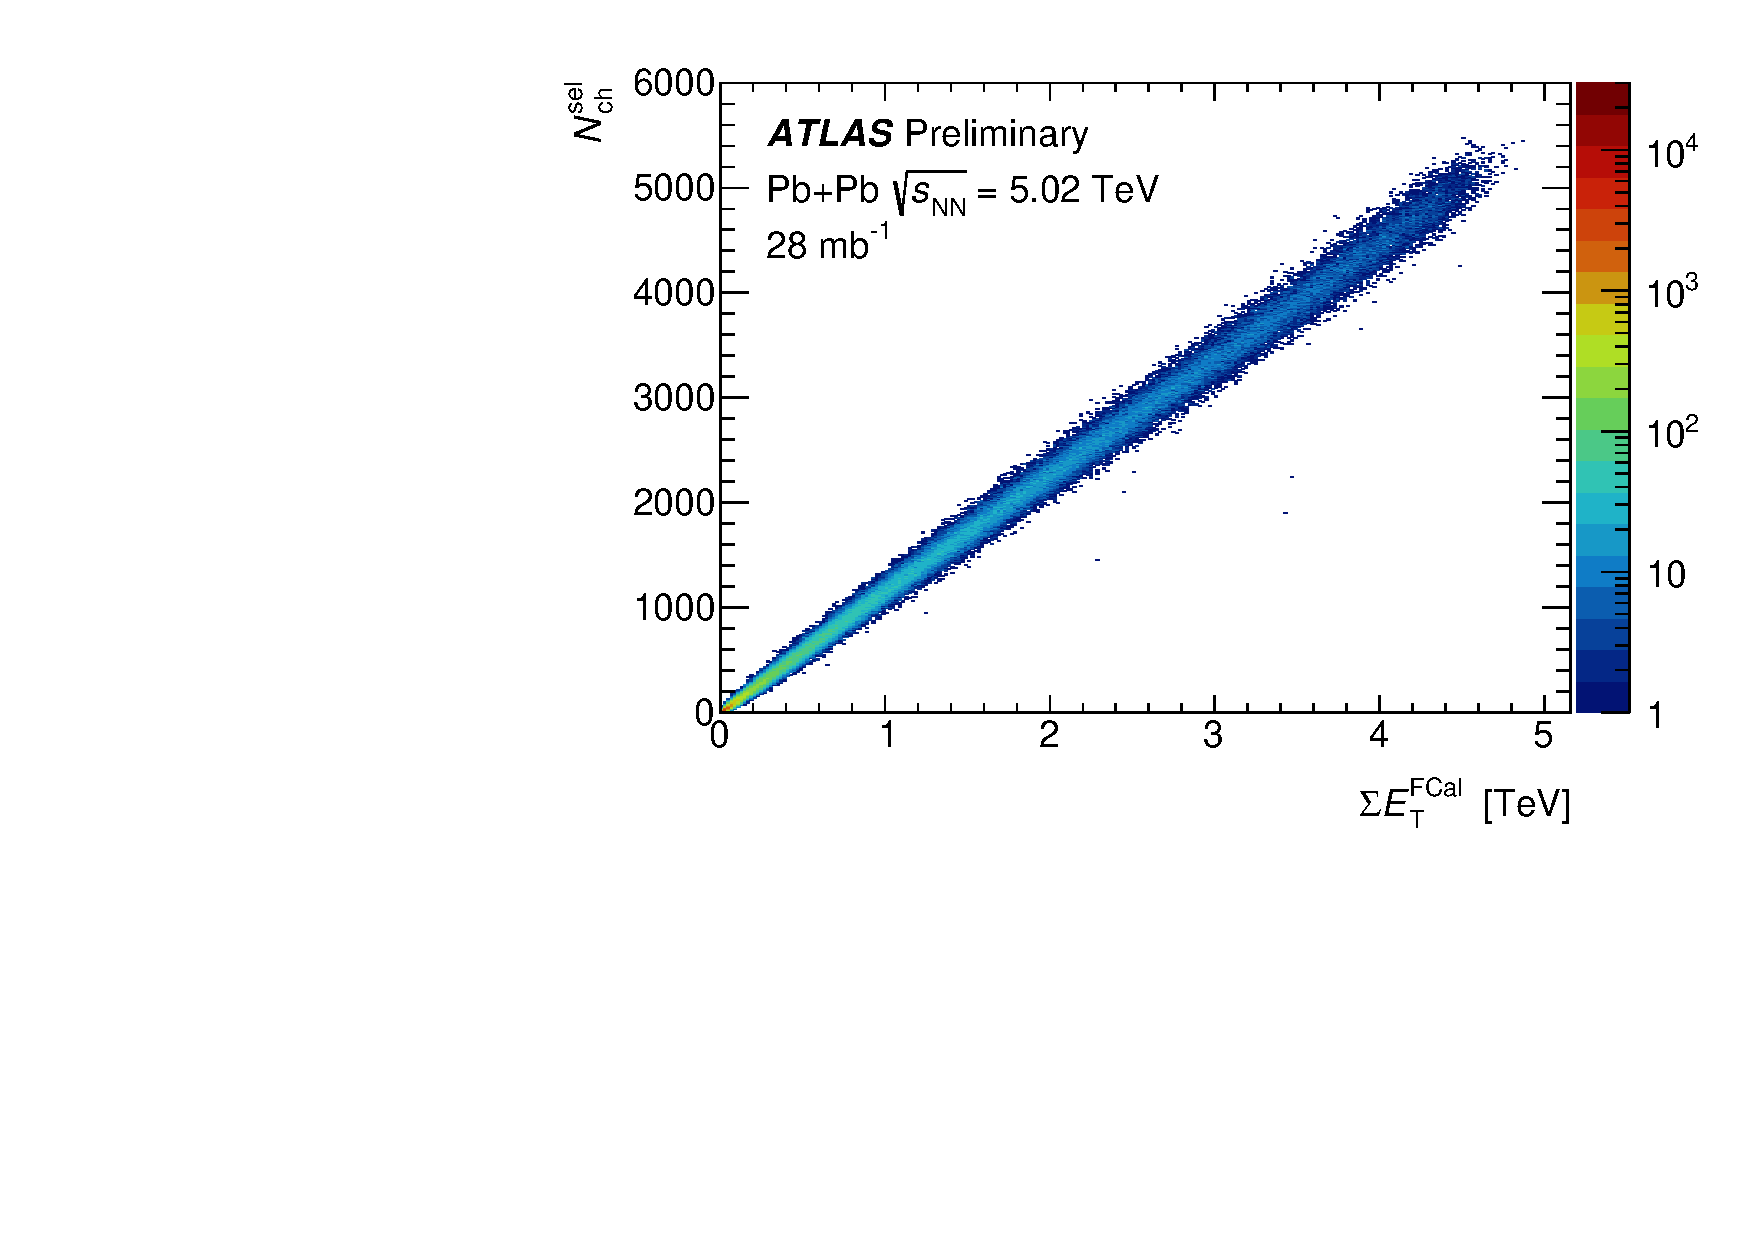
\includegraphics[width=\linewidth]{figures/setup/nch_fcal}
          \caption{}
          \label{fig:nch_fcal}
\end{subfigure}
\qquad  \qquad  
\begin{subfigure}{.45\textwidth}  
  \centering
  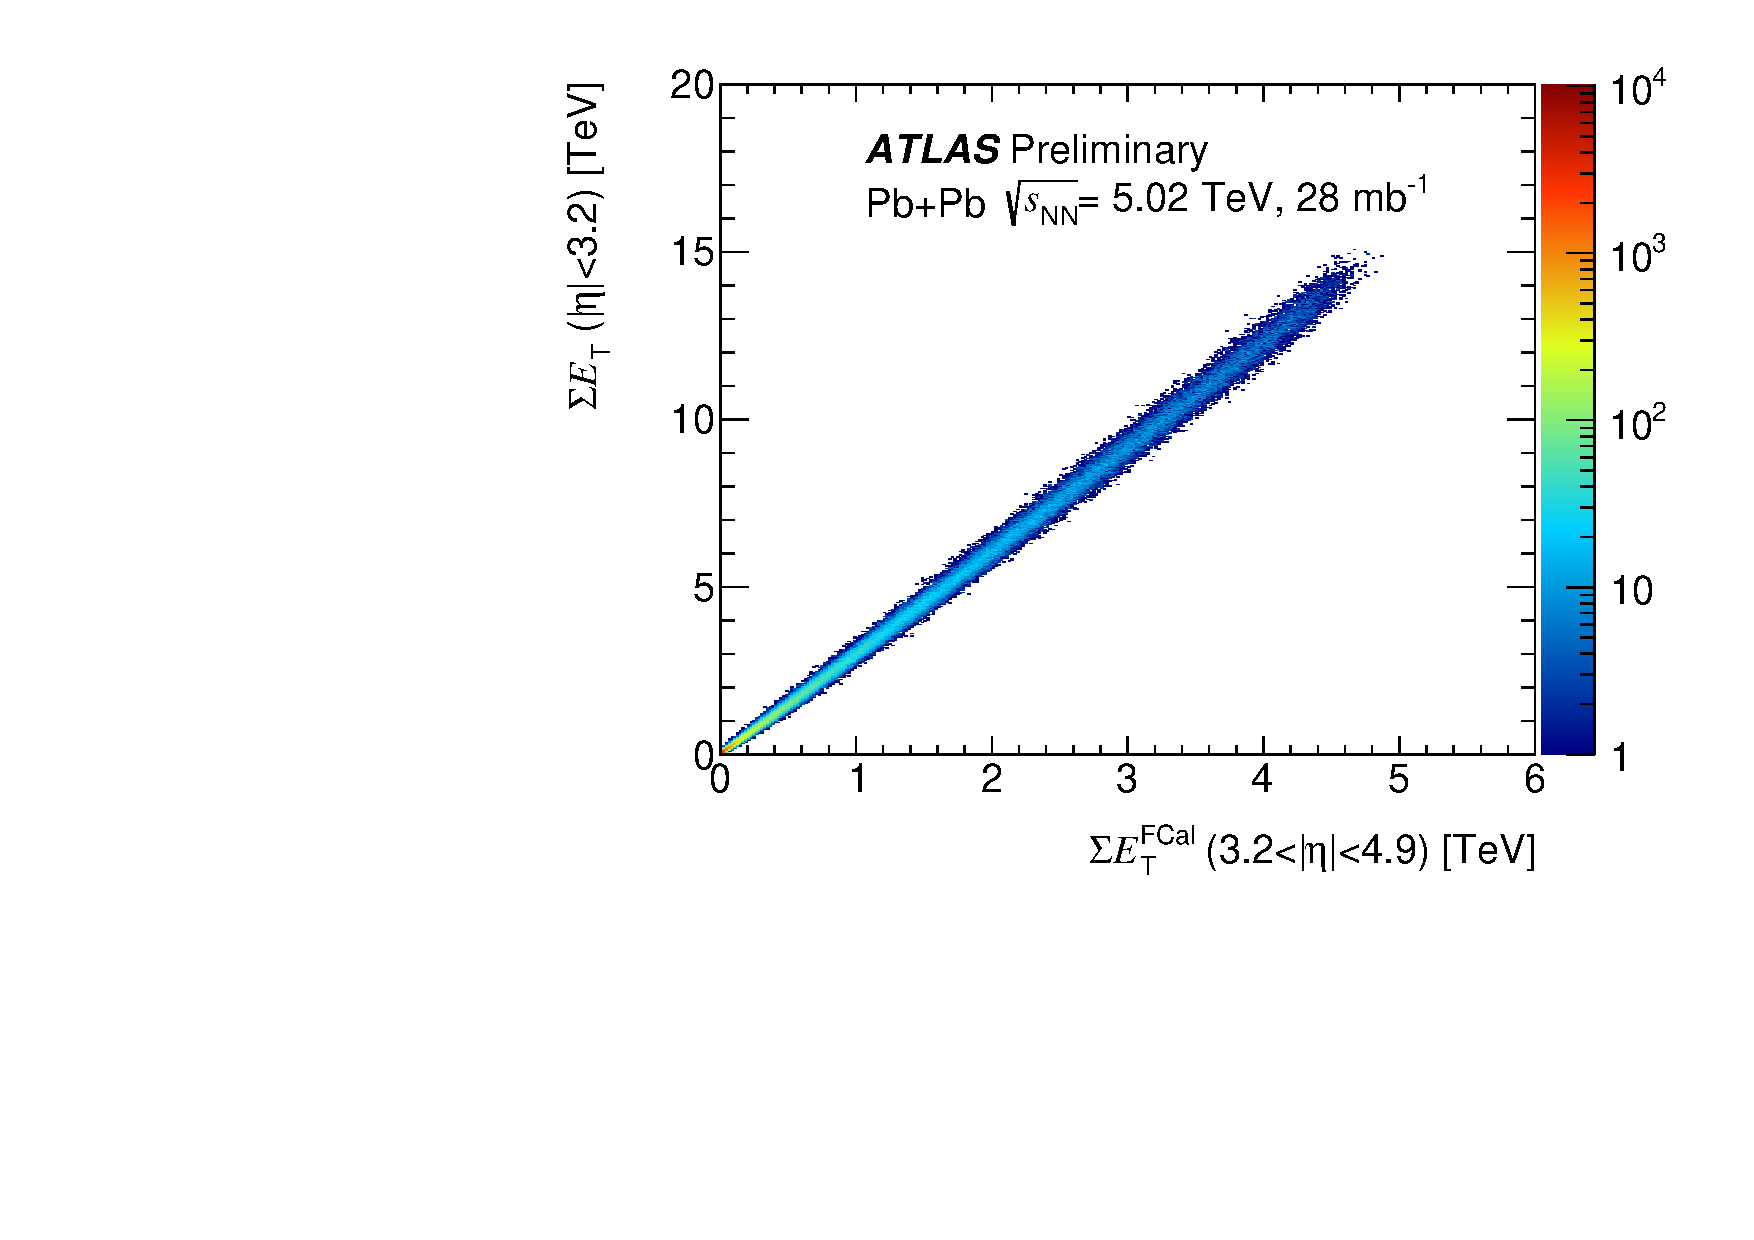
\includegraphics[width=\linewidth]{figures/setup/fcal_barrel}
          \caption{}
          \label{fig:fcal_barrel}
\end{subfigure}
\caption{(Left) Number of reconstructed charged particles $\Nch^{\rm sel}$ versus the total transverse energy in the FCal, \ETfcal.
(Right) Correlation of the total energy in the calorimeter in the interval of $|\eta| < 3.2$ with the total energy measured in the forward calorimeters.
Both plots are for \pbpb\ collisions with \sqrtsnn = 5.02 TeV.
Taken from Ref.~\cite{perfPlots}.}
\label{fig:jetcs}
\end{figure}



\begin{figure}[ht]
	\centering
        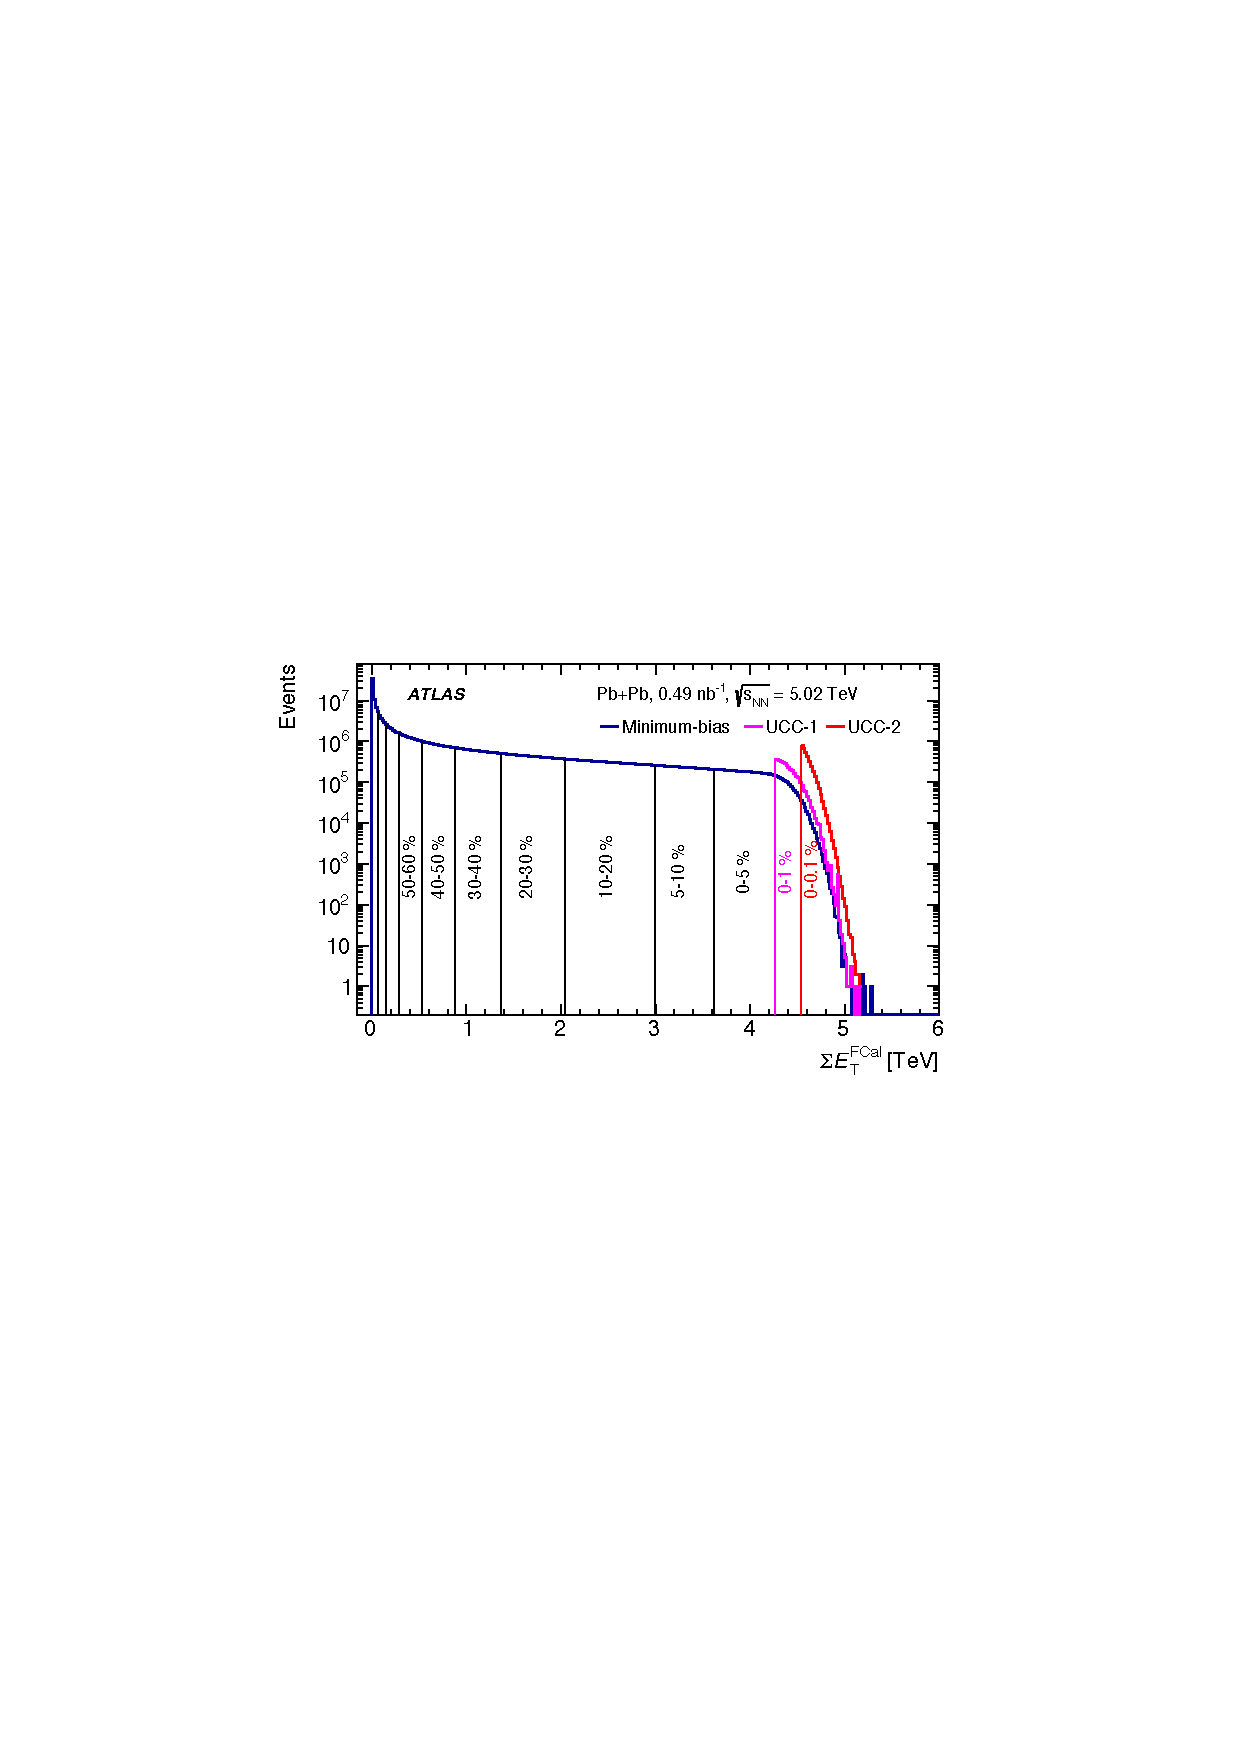
\includegraphics[width=0.5\textwidth]{figures/setup/fcal_distr}
          \caption{The \ETfcal\ distribution in $\sqrtsnn = 5.02$ TeV \pbpb\ collisions for events selected by the minimum bias trigger.
          The \ETfcal\ thresholds for several centrality intervals are marked with vertical lines and labelled on the plot.
           Also shown are the number of events over the 0--1\% and 0--0.1\% centrality intervals selected by the ultra-central triggers.
           Figure taken from Ref.~\cite{Aaboud:2018ves}.}
          \label{fig:fcal_distr}
\end{figure}


\section{Jet Reconstruction for Heavy Ion Collisions in ATLAS}
% !TEX root = thesis-ex.tex
Of the jet reconstruction algorithms that were discussed in Section~\ref{sec:jet_algo}, the LHC collaborations use the \antikt\ algorithm.
The ATLAS jet reconstruction procedure in heavy ion collisions is described in Ref.~\cite{2019108}, and is summarized in Figure~\ref{fig:atlasHIjetreco}.
It is different from the procedure for \pp\ collisions because of the large underlying event present in the heavy ion collision system.
%The heavy ion jet reconstruction procedure however, can also be applied to \pp\ collisions with ,

\begin{figure}[htbp!]
	\centering
	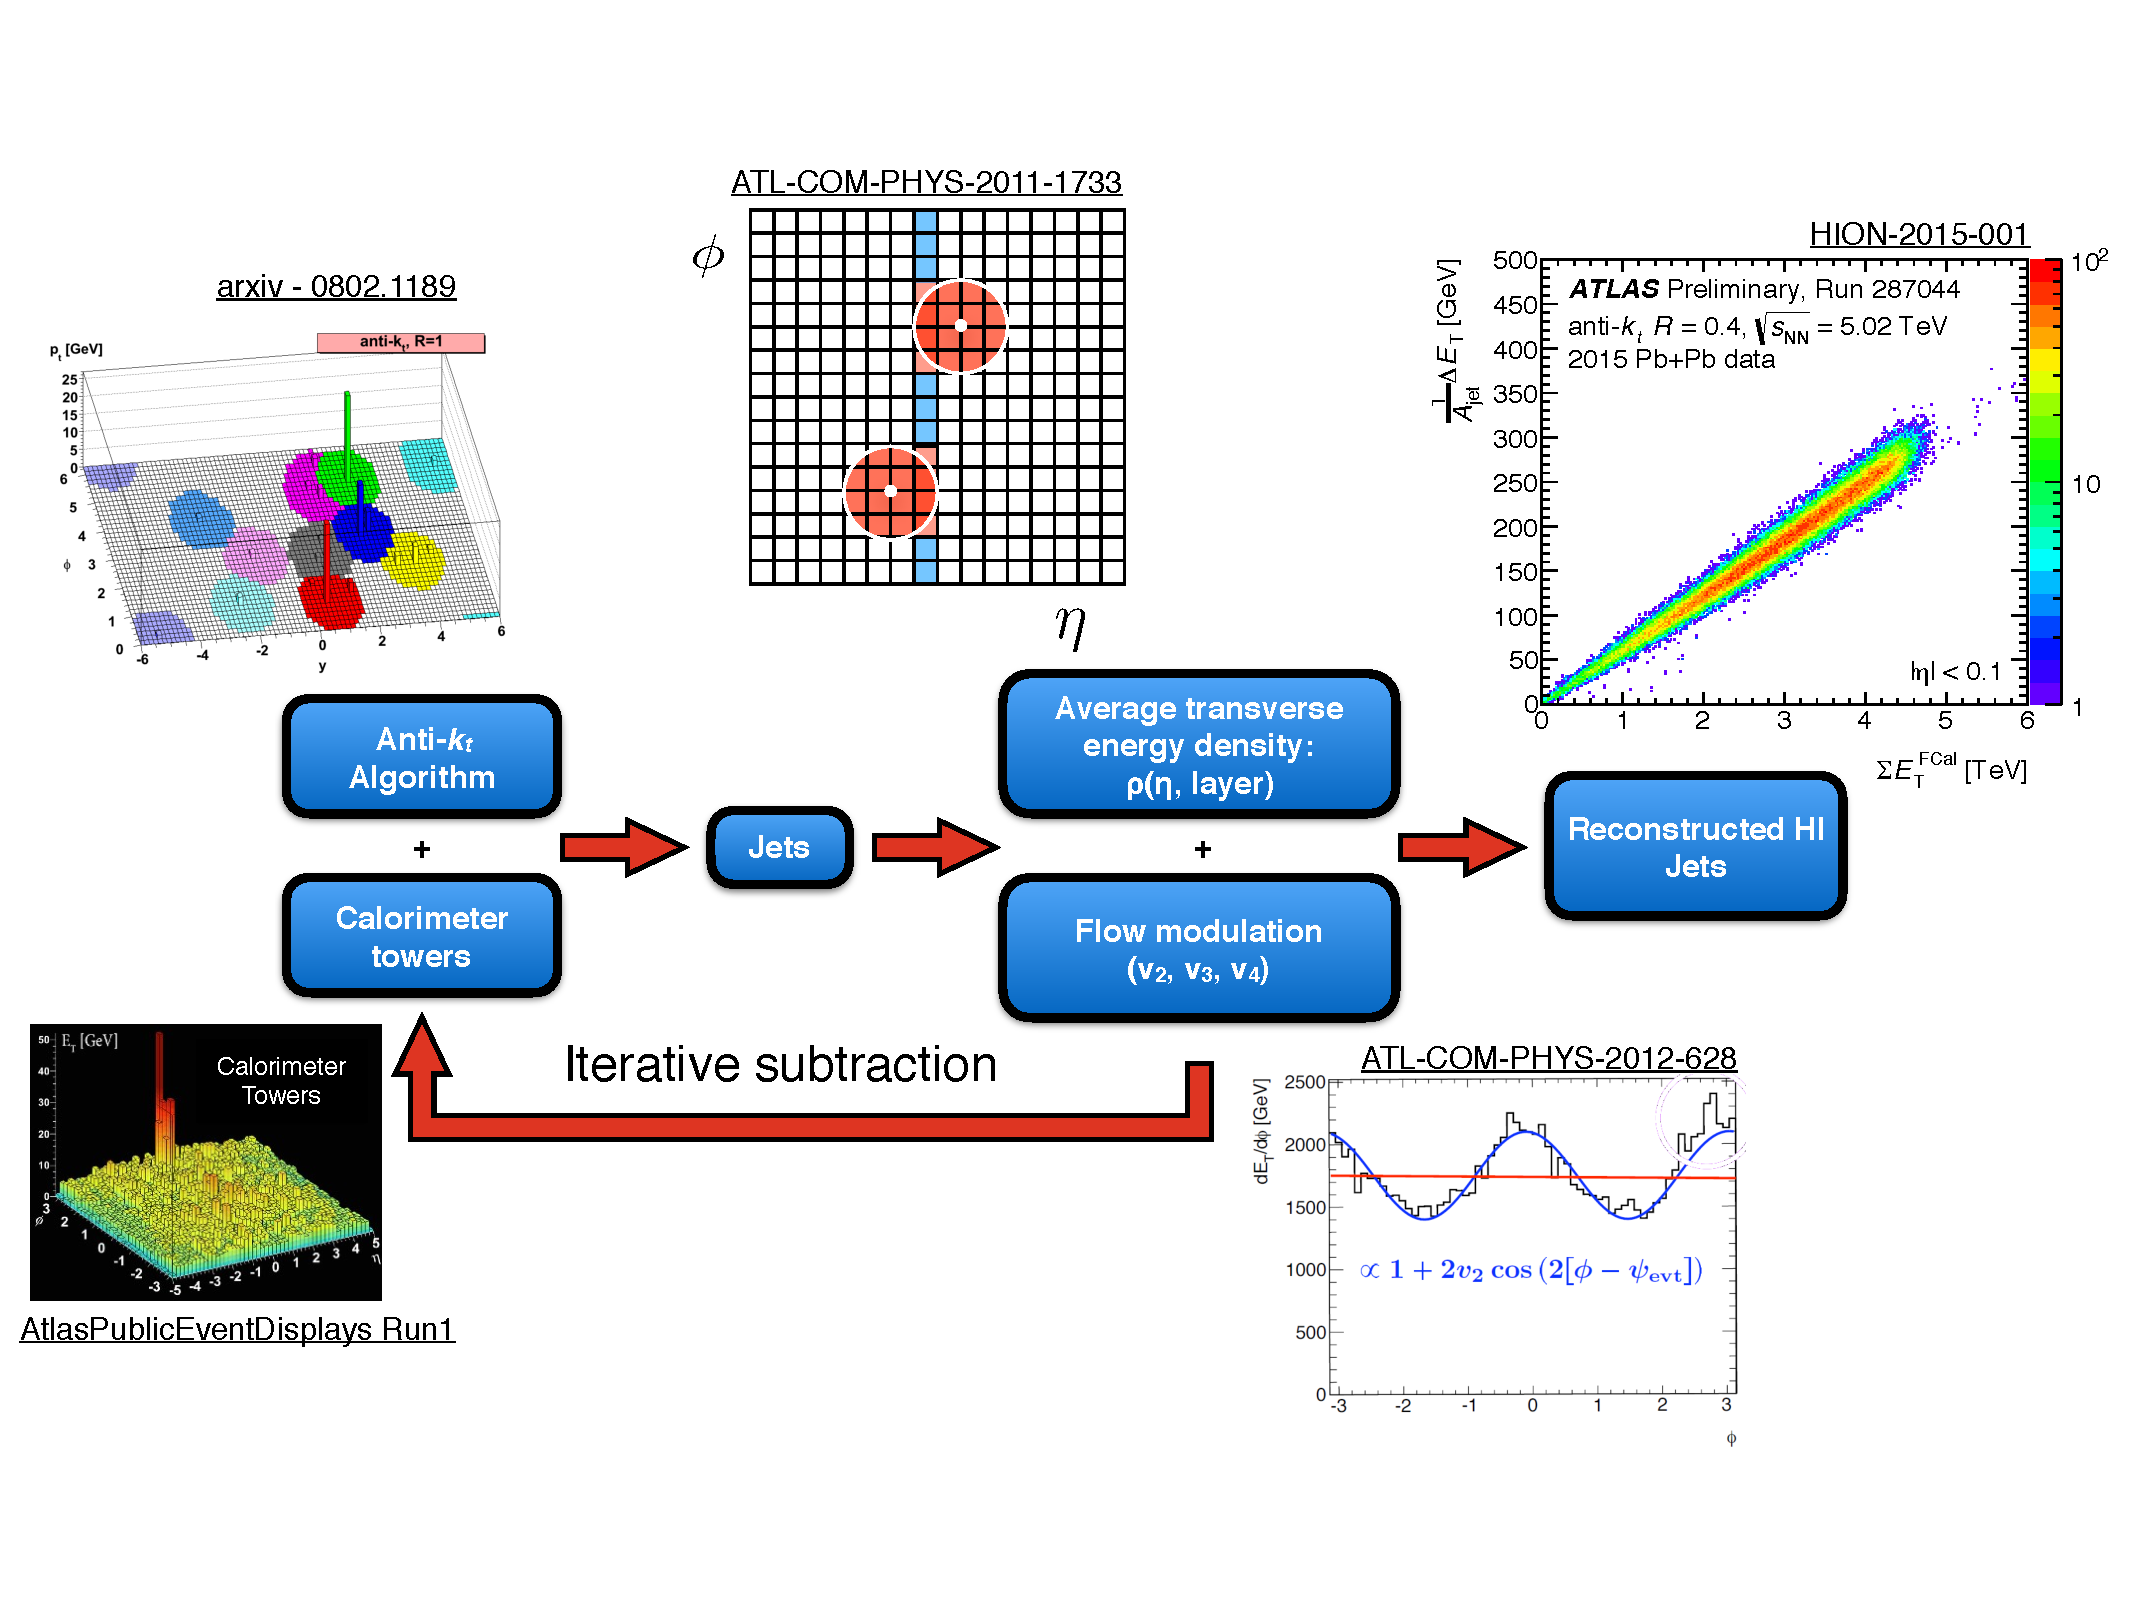
\includegraphics[width=0.7\textwidth]{figures/setup/atlasHIjetReco} %
	\caption{A schematic of the ATLAS jet reconstruction procedure.
	Inset figures from Refs.~\cite{Cacciari:2008gp, atlasRun1EventDisplay, ATLAS-COM-PHYS-2011-1733, Cole:1450219, perfPlots}.}	
	\label{fig:atlasHIjetreco}%
\end{figure}

This procedure uses the \antikt\ algorithm as implemented in \textsc{FastJet} software package \cite{fastjet_algo}.
The \antikt\ algorithm is run in four-momentum recombination mode with its inputs being the $\eta \times \phi = 0.1 \times \pi / 32$ calorimeter towers.
The tower energies are the sum of the energies of all layers in the tower with cells that straddle tower boundaries having their energies fractionally distributed.
The \antikt\ algorithm is first run with the distance parameter $R=0.2$, to give seed jets.

These seed jets contain at least one tower with $\Et > 3$ GeV, and have the ratio of the maximum tower transverse energy to the average tower transverse energy, $\Et^{Max} / \langle \Et \rangle > 4$.
Then the underlying event subtraction procedure is performed.
A first estimate of the average underlying event energy density $\rho_i (\eta)$ is done in 0.1 slices of $\eta$ in each calorimeter layer $i$ after excluding the regions that overlap with the seed jets.
A modulation is applied to account for the flow from the QGP (discussed in Section~\ref{sec:qgp_hi}) and the underlying event is subtracted to give $E_{Tj}^{\mathrm{sub}}$:

\begin{align}
E_{Tj}^{\mathrm{sub}} = E_{Tj} - A_j \rho_i (\eta_j) \Big(1+2 \sum_{n=2}^{4} {v_{n}}_i \big(\cos[2(\phi_j-\Psi_n)] \big) \Big)
\end{align}
where $E_{Tj} , \eta_j, \phi_j$ and $A_j$ are the cell $E_T, \eta, \phi$ and area for cell $j$ in layer $i$.
$v_{ni}$ are the $n^{\rm th}$ order harmonics of the modulation in layer $i$and are given by:

\begin{align}
v_{ni} = \frac{\sum_{j \in i} \Et_j \cos[2(\phi_j-\Psi_n)]}{\sum_{j \in i} \Et_j}
\end{align}
where the sum is over all cells $j$ in layer $i$.
$\Psi_n$ is the event plane angle and is given by \cite{ATLAS:2012at}:

\begin{align}
\Psi_n = \frac{1}{n} \tan^{-1} \left[ \frac{\langle \sum_k w_k \Et_k \sin(n\phi_k) \rangle}{\sum_k \Et_k \sin(n\phi_k)} \right]
\end{align}
where the sum is over all $k$ cells in the FCal and $\phi_k$ is the azimuthal angle of the cell.
The $w_k$ weights are to ensure a uniform $\Psi_n$ distribution.
The dominant effect in the modulation is from the second and third harmonic, $v_2$ and $v_3$ \cite{ATLAS:2012at}.

Once the background is subtracted, the \antikt\ algorithm is run again with the distance parameter $R = 0.2$.
The underlying event is re-estimated after excluding areas that are within $\Delta R = 0.4$ of the seeds.
Updated values of $\rho{'}_i$ and $v{'}_2$ are recalculated and used to estimate the background that is subtracted from the original cell energies.
This is then subtracted from the original cell energies to give kinematics for the $R= 0.4$ jets.
The average subtracted energy normalized by the area of the jet reconstructed jet, as a function of the energy in the forward calorimeter is shown in Fig~\ref{fig:subtr_energy}.
It can be seen that in the barrel region for $|\eta| < 0.1$, $R=0.4$ jets have a background that is approximately $300/(\pi\times 0.4^2) \approx 150$ GeV.
Figure~\ref{fig:jet_event_display} shows an ATLAS event display for a heavy ion collision with a reconstructed jet.


\begin{figure}
\centering
  \begin{minipage}{0.45\textwidth}
	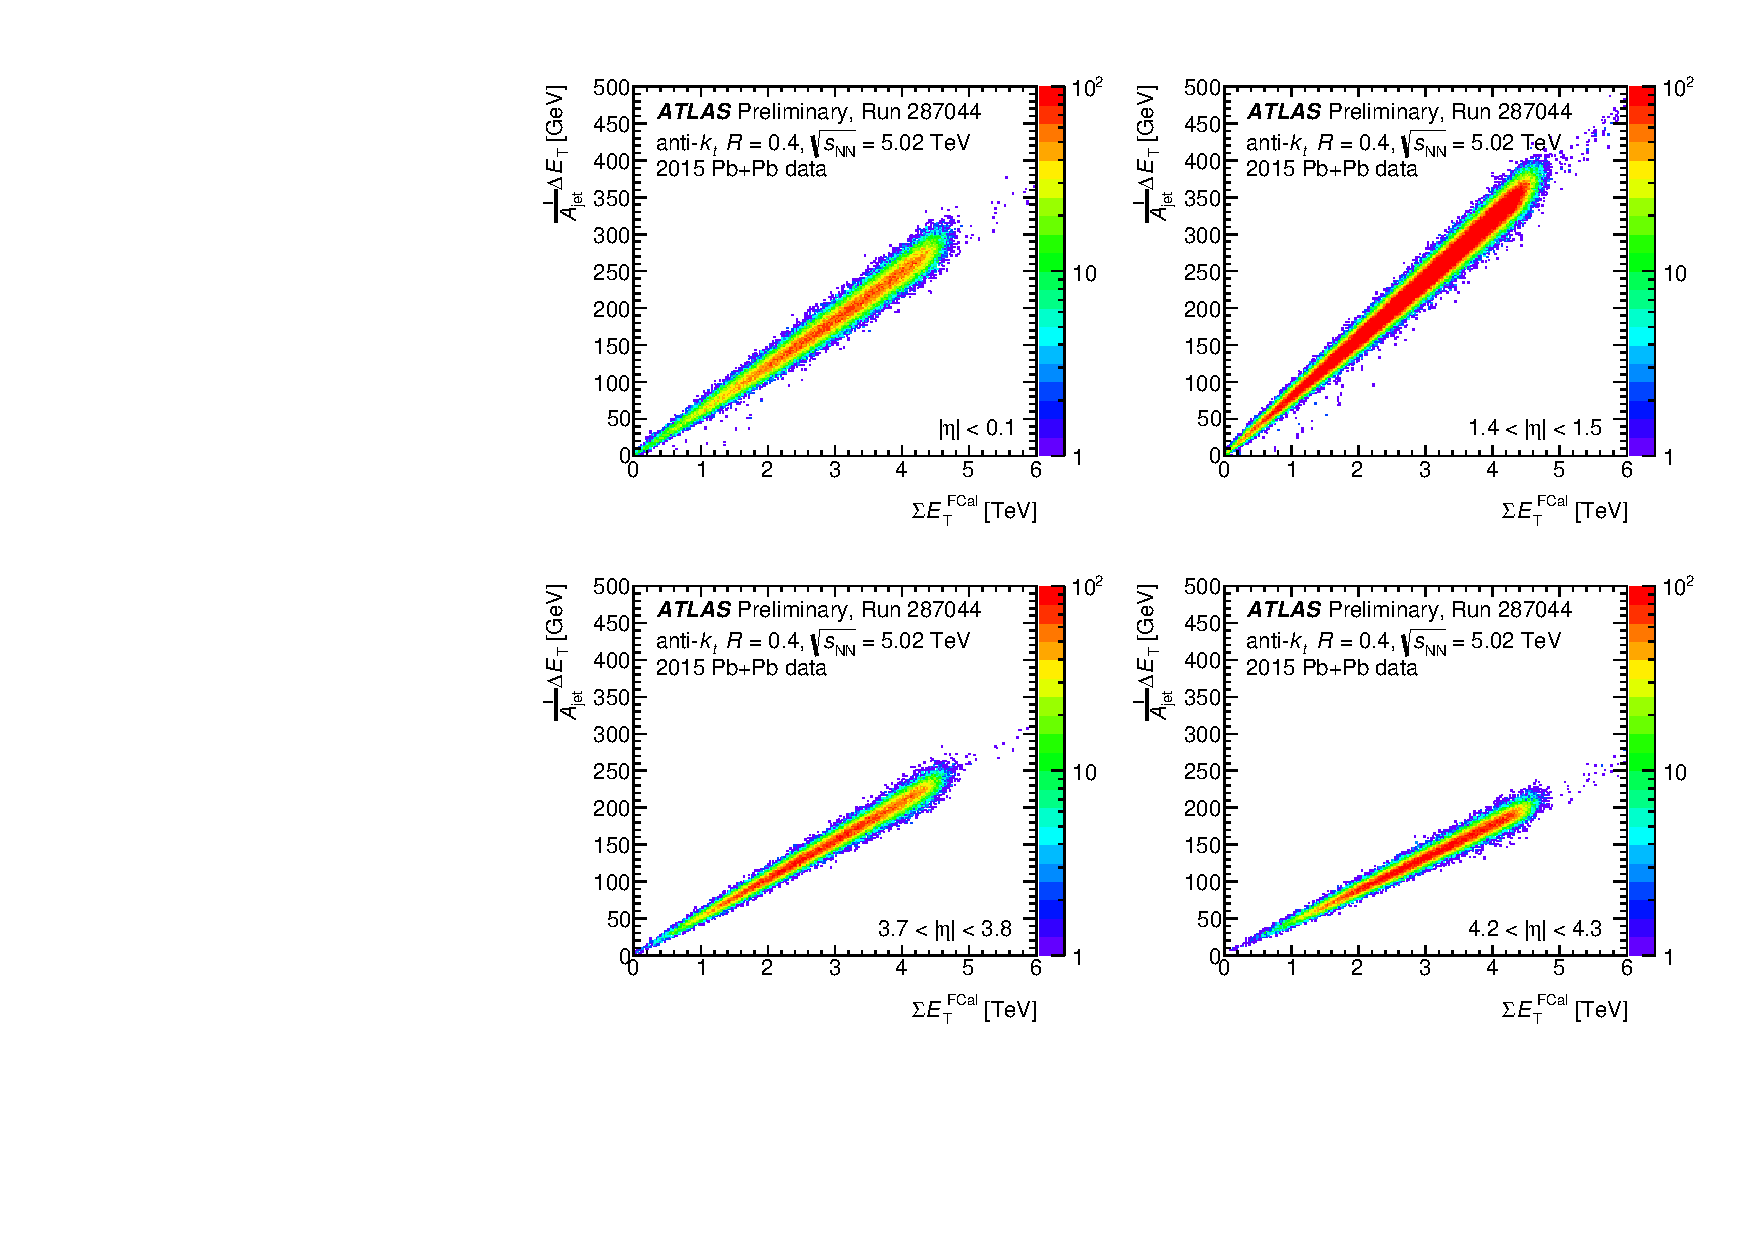
\includegraphics[width=1.\textwidth]{figures/setup/subtr_energy} %
	\caption{The subtracted transverse energy $\Delta \Et$, normalized by the jet area $A_{\rm{jet}}$ as a function of \ETfcal\ in \pbpb\ collisions at $\sqrtsnn = 5.02$ TeV.
	Figure from Ref.~\cite{perfPlots}.}	
	\label{fig:subtr_energy}
  \end{minipage}
 \qquad 
  \begin{minipage}{0.43\textwidth}
	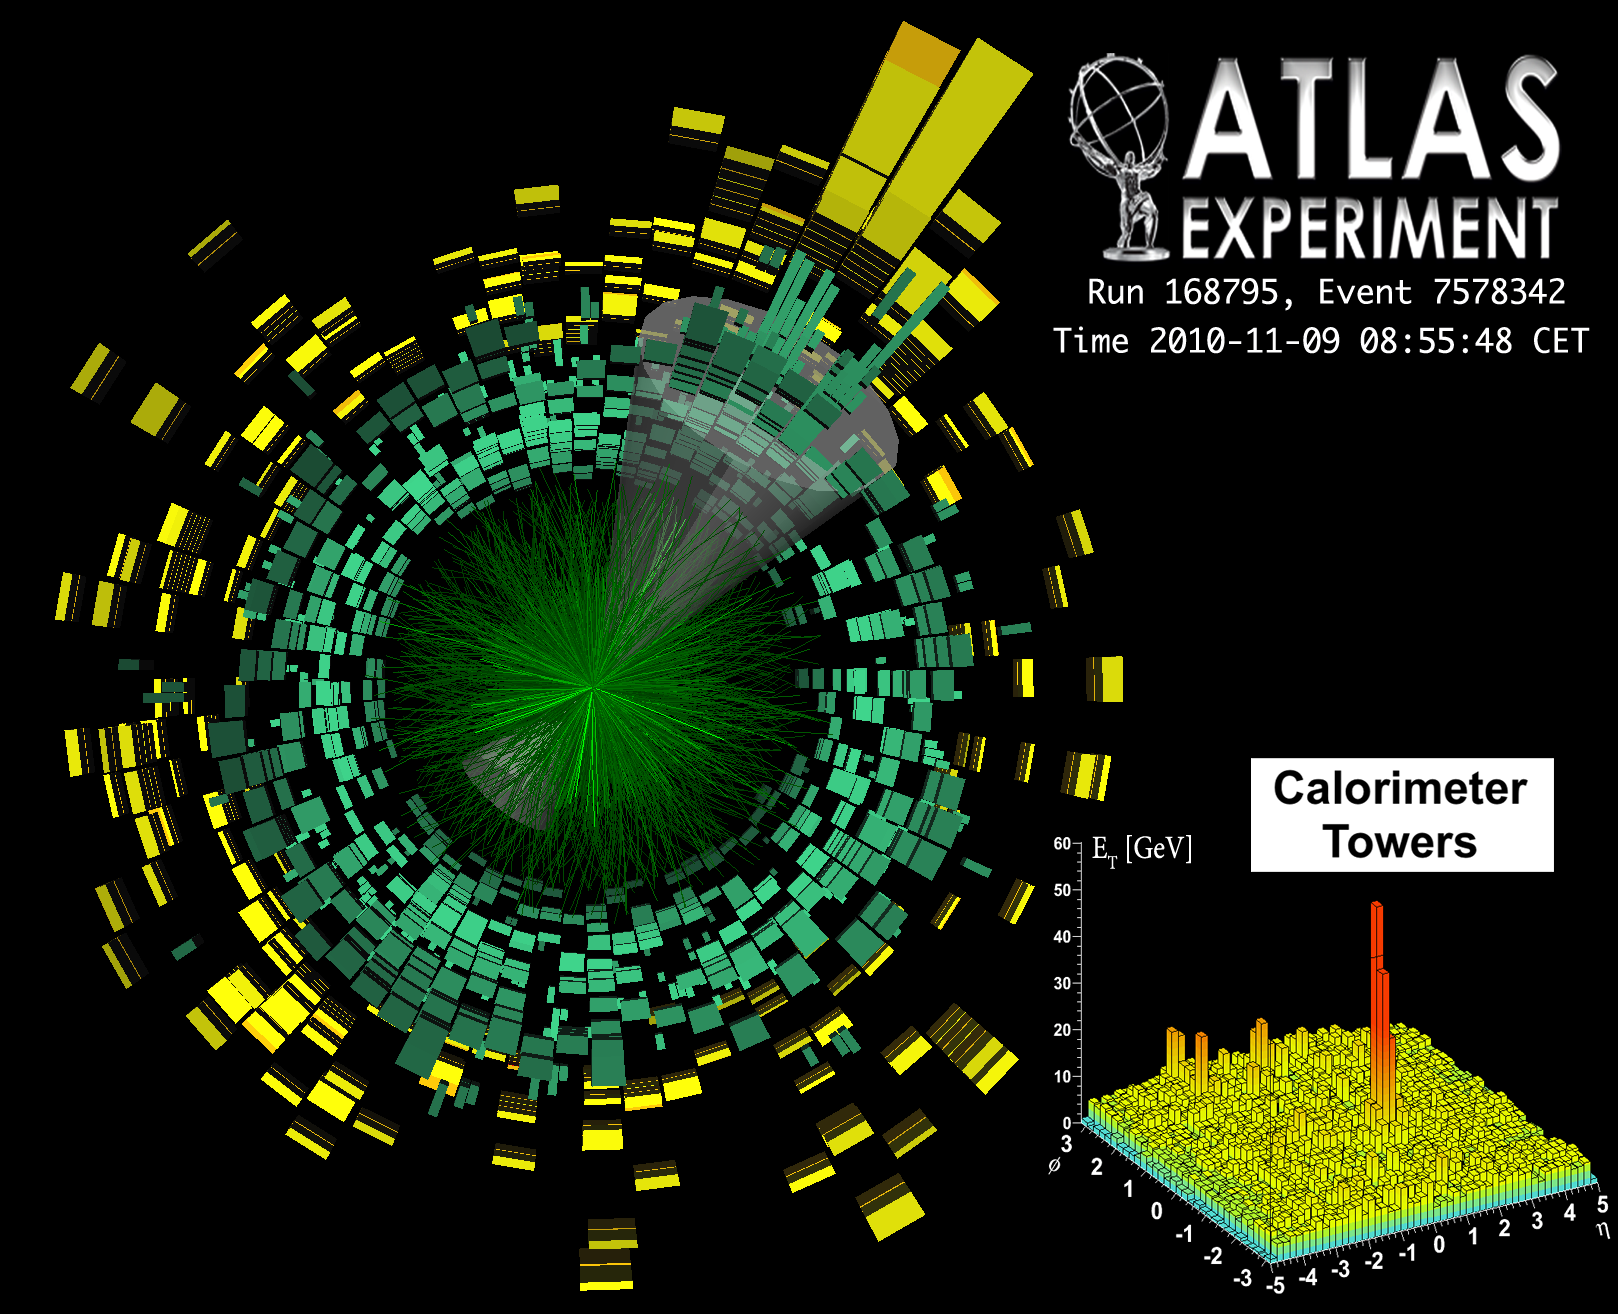
\includegraphics[width=1.\textwidth]{figures/setup/jet_event_display} %
	\caption{
	An asymmetric dijet event in \pbpb\ collisions at \sqrtsnn = 2.76 TeV as measured by the ATLAS detector. 
	Figure from Ref.~\cite{atlasRun1EventDisplay}.}	
	\label{fig:jet_event_display}
  \end{minipage}
\end{figure}



%
%\begin{figure}[htbp!]
%	\centering
%	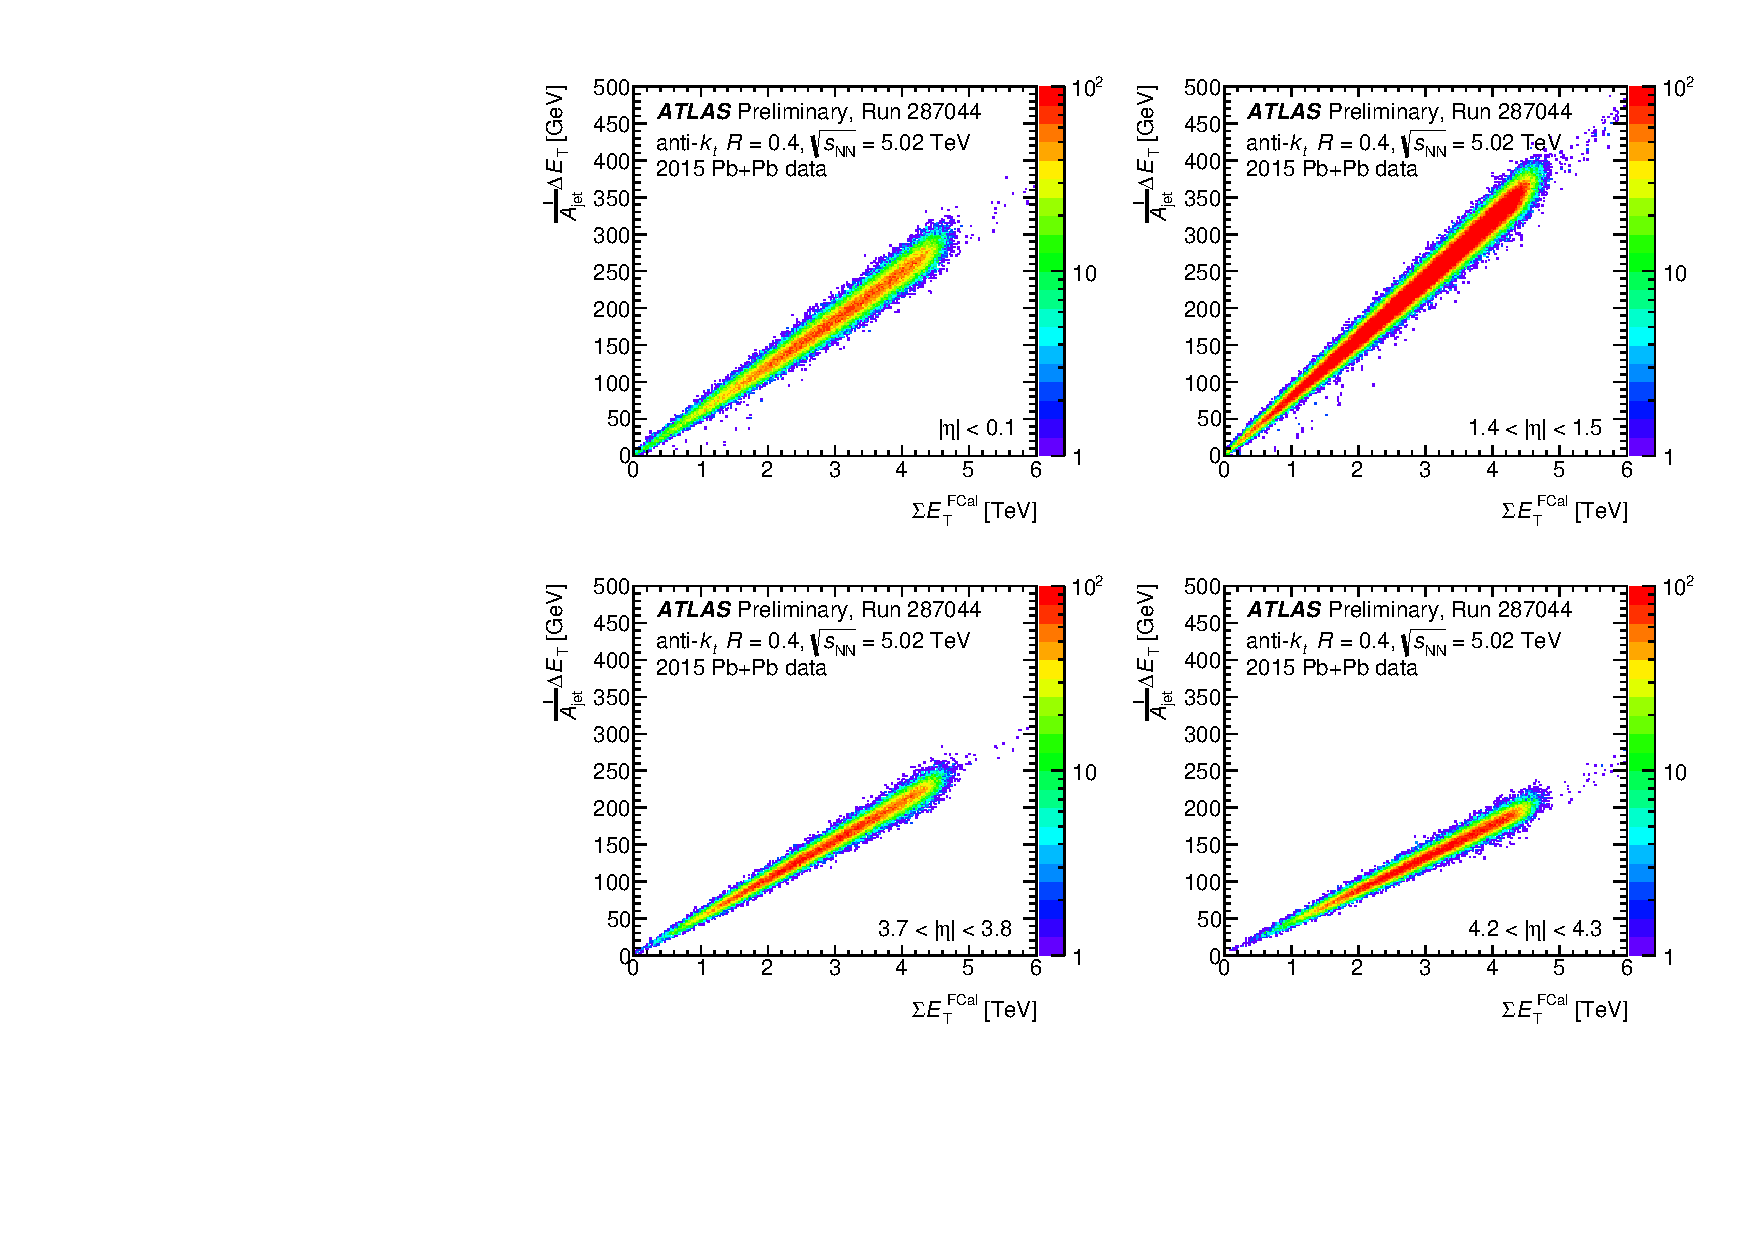
\includegraphics[width=0.5\textwidth]{figures/setup/subtr_energy} %
%	\caption{
%	The subtracted transverse energy $\Delta \Et$, normalized by the area of the jet $A_{\rm{jet}}$ as a function of the sum of the energy deposited in the forward calorimeter $\sum \Et_{\rm FCal}$ in \pbpb\ collisions at $\sqrtsnn = 5.02$ TeV.
%	The jets were reconstructed using the \antikt\ algorithm with $R = 0.4$.
%	Four panels show four selections on the pseudorapidity of the jet.
%	Figures taken from Ref.~\cite{perfPlots}.}	
%	\label{fig:subtr_energy}
%\end{figure}
%
%
%\begin{figure}[htbp!]
%	\centering
%	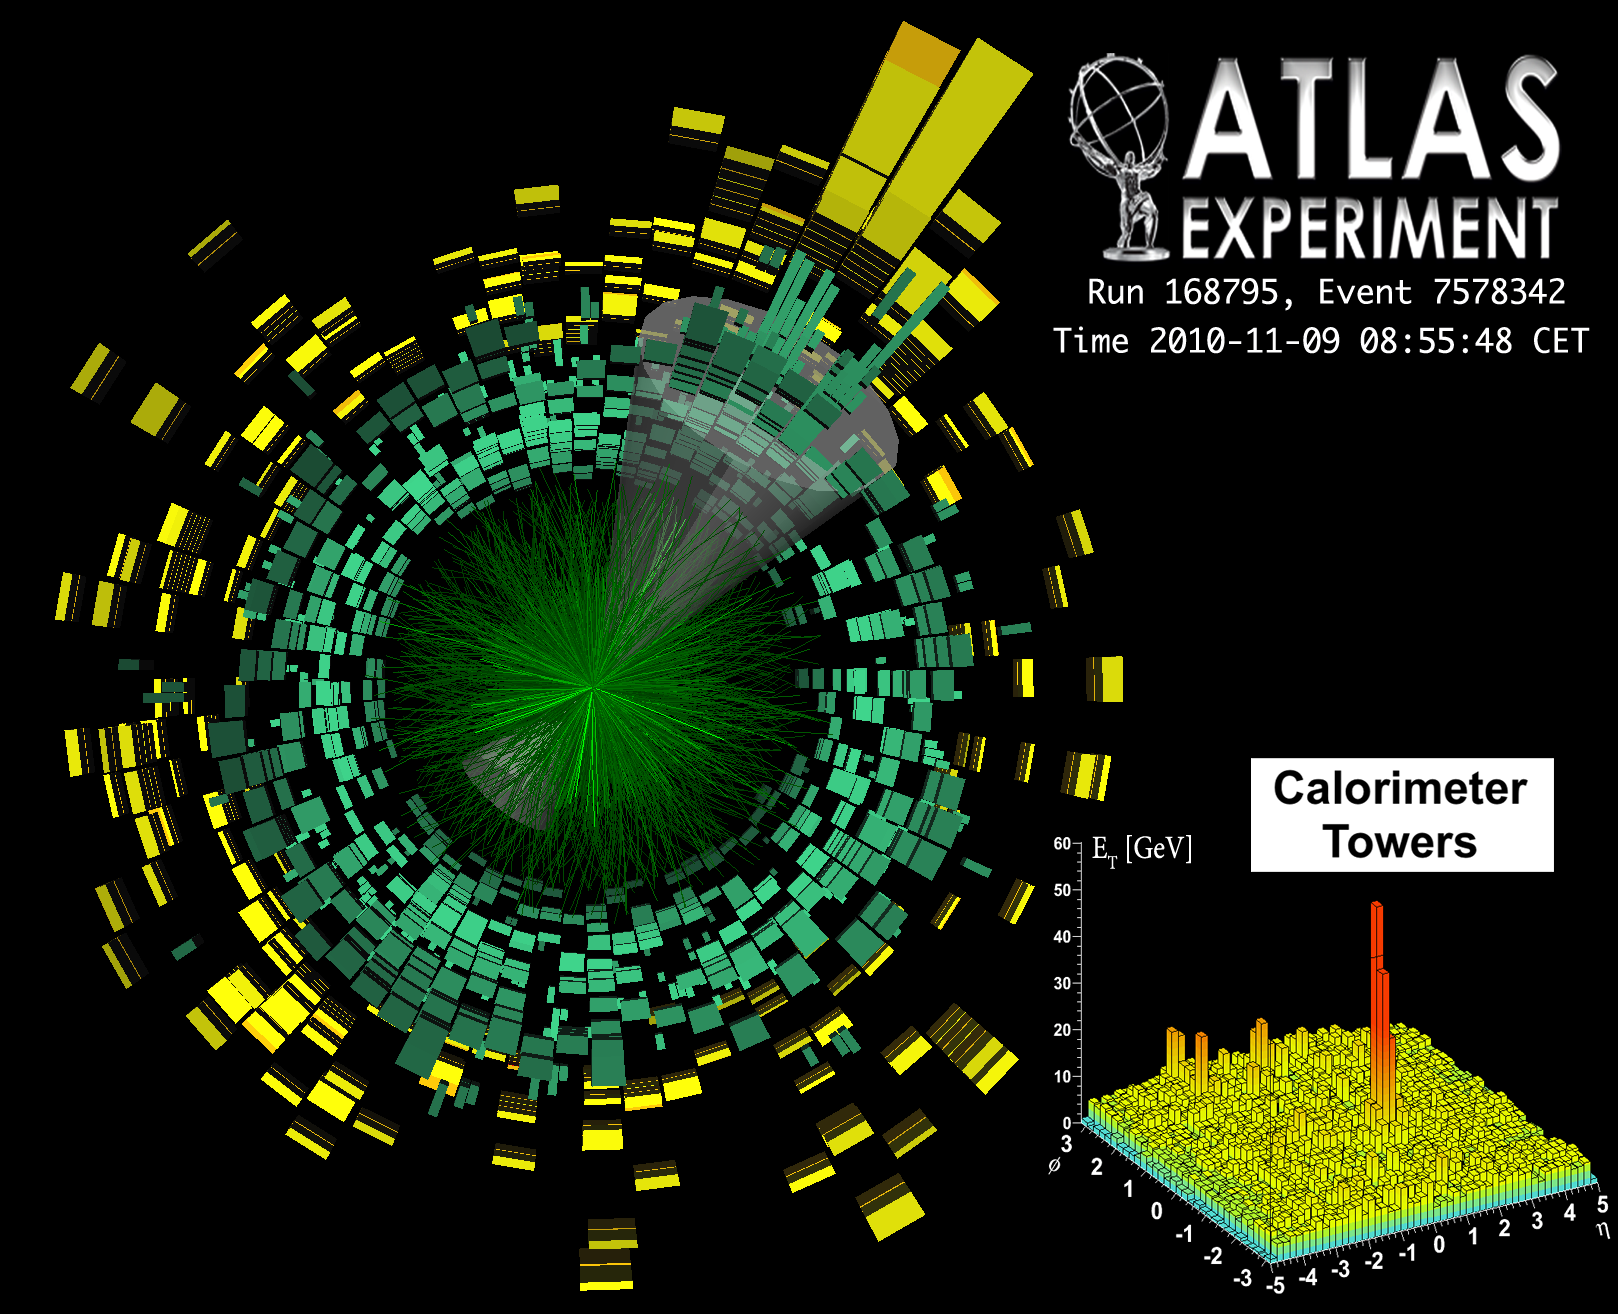
\includegraphics[width=0.5\textwidth]{figures/setup/jet_event_display} %
%	\caption{
%	An asymmetric dijet event in \pbpb\ collisions at \sqrtsnn = 2.76 TeV as measured by the ATLAS detector. 
%	Figures taken from Ref.~\cite{atlasRun1EventDisplay}.}	
%	\label{fig:jet_event_display}
%\end{figure}



\section{Jet Calibration for Heavy Ion Collisions in ATLAS}
% !TEX root = thesis-ex.tex

The hadronic shower (jet) has both electromagnetic and non-electromagnetic components that interact with the calorimeter material differently.
Thus the energy response of the calorimeter for these components is different (this is called a non-compensating calorimeter \cite{calorimetry_book}), and hence, calibrations are required to correct the reconstructed jet kinematics.
These take into account features of the detector, the reconstruction algorithm, and jet fragmentation and include the following \cite{Aad:2014bia}:
\subparagraph{Origin Correction: } This correction ensures that jets point back to the primary vertex and not the nominal center of the detector.
\subparagraph{MC based Calibration: } This is a MC based correction that depends on the comparison between the energy and pseudorapidity of the reconstructed jet and the corresponding matched truth jet.
\subparagraph{\textit{In situ}+Cross Calibration: } This calibration is based on the differences between data and MC as described by a well-measured object like a photon or Z boson.
This poses a challenge for heavy ion collisions because unlike in \pp\ collisions, there simply aren't enough statistics for these objects.
Here the cross-calibration procedure accounts for differences in the jet reconstruction procedure in heavy ion collisions and \pp\ collisions, and enables the usage of the \insitu\ corrections from \pp\ collisions.

The validity of the jet reconstruction and calibration procedure can be tested by evaluating the jet energy scale and jet energy resolution.
These are the mean and width respectively of the jet response distribution that is given by $\ptreco / \pttruth$ in MC and are shown in Figure~\ref{fig:jes_jer}.
\ptreco\ is the reconstructed jets transverse momentum, while \pttruth\ is the transverse momentum of the corresponding ``truth'' jet.


\begin{figure}[htbp!]
	\centering
	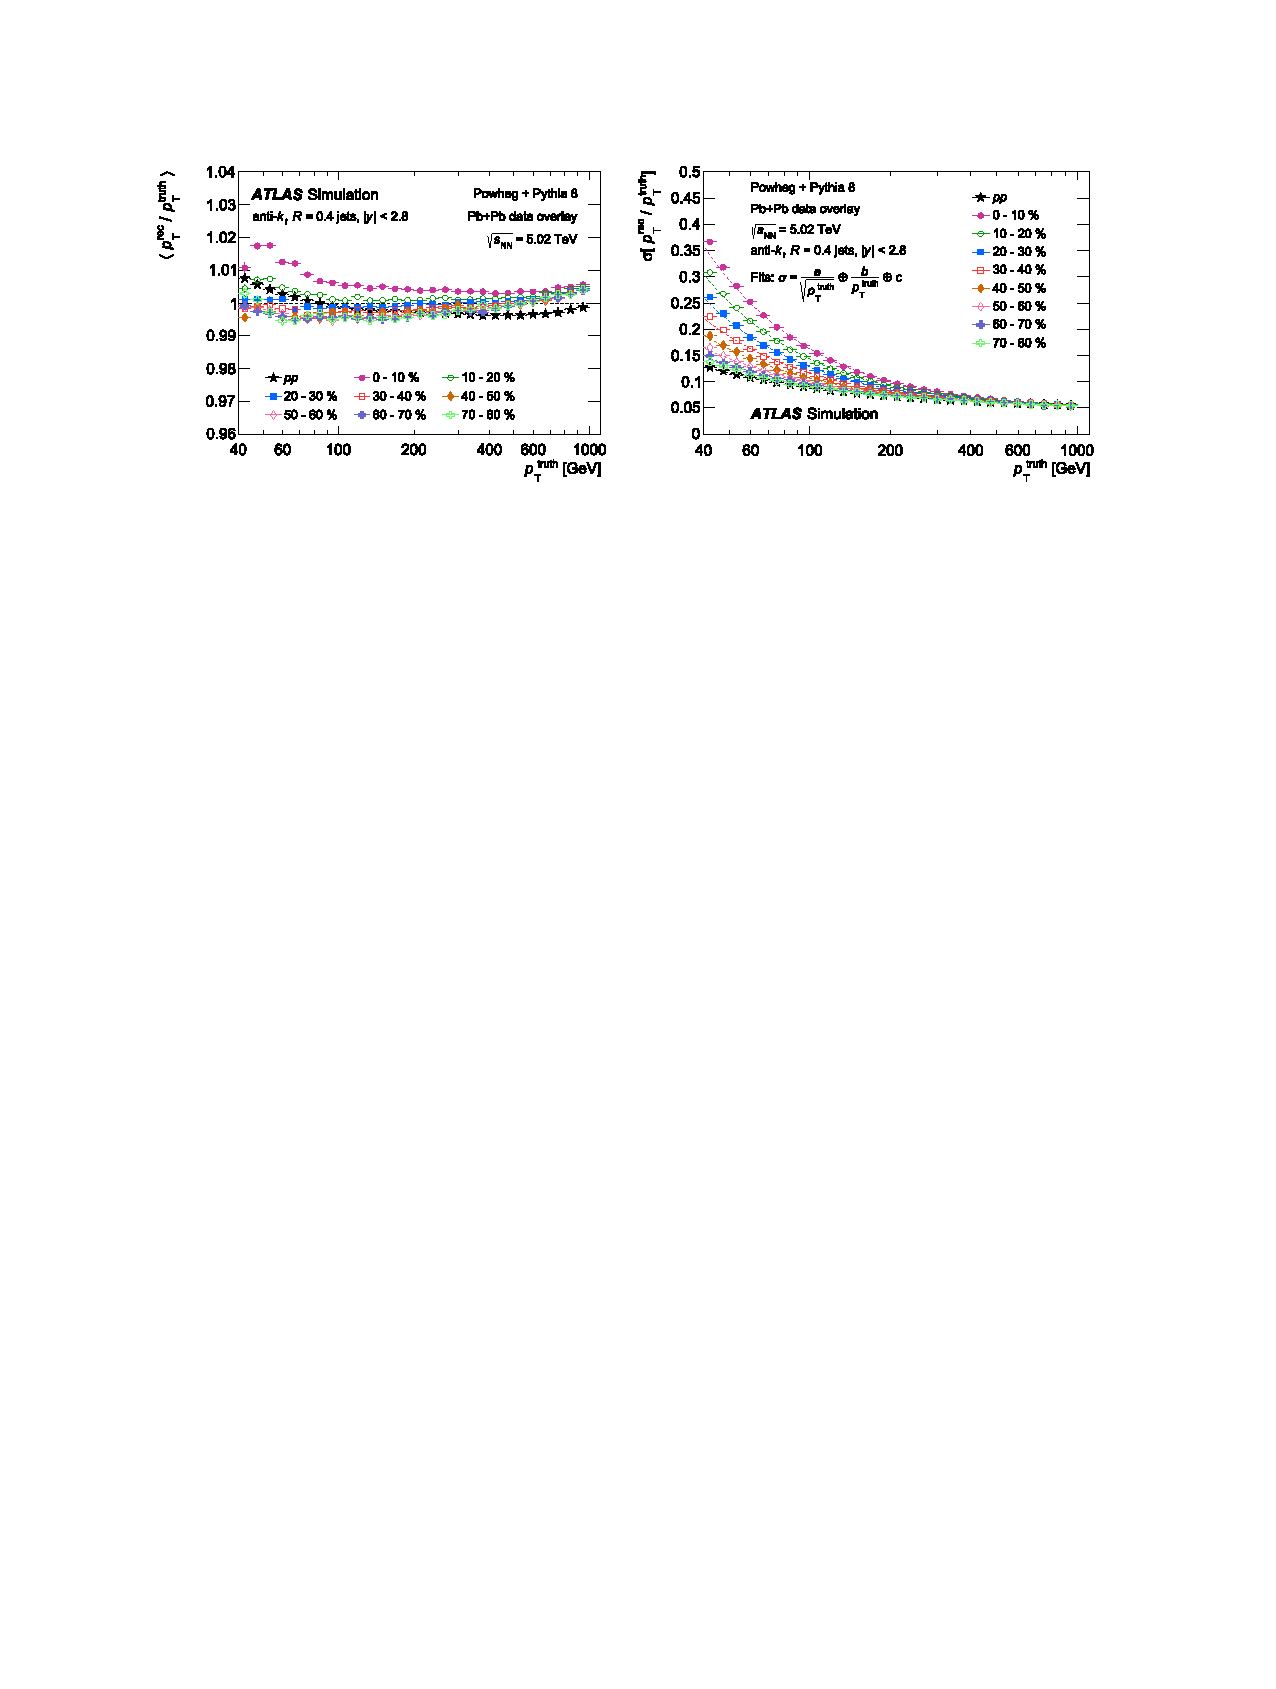
\includegraphics[width=\textwidth]{figures/setup/jes_jer} %
	\caption{
	The Jet Energy Scale (left) and Jet Energy Resolution (right) as a function of \pttruth.
	Both are for jets with $|y| < 2.8$. The different curves are for \pp\ and varying \pbpb\ centrality.
	Figures taken from \cite{2019108}.}	
	\label{fig:jes_jer}%
\end{figure}
The JES is seen to be almost unity within 1\%. across a broad kinematic range.
The JER is smaller for jets with higher transverse momentum, and depends on centrality.
It is the largest in central collisions and gets better for more peripheral collisions.
The JER can be fit to the form \cite{Aad:hi_jets}:

\begin{align}
\frac{\sigma[\Delta \Et]}{E_{\rm T}^{\rm true}} = \frac{a}{\sqrt{E_{\rm T}^{\rm true}}} \oplus \frac{b}{E_{\rm T}^{\rm true}} \oplus c
\end{align}
where $a$ and $c$ are related to the detector response.
The $b$ term describes the underlying event fluctuations and depends on centrality.
The large underlying event in central collisions results in the JER being the largest in that centrality interval. 

The $\eta$ and $\phi$ position resolution of the jet can be derived via a similar procedure and is shown in Figure~\ref{fig:jet_posResolution} as a function of the \pttruth.



\begin{figure}
\centering
\begin{subfigure}{.45\textwidth}
  \centering
  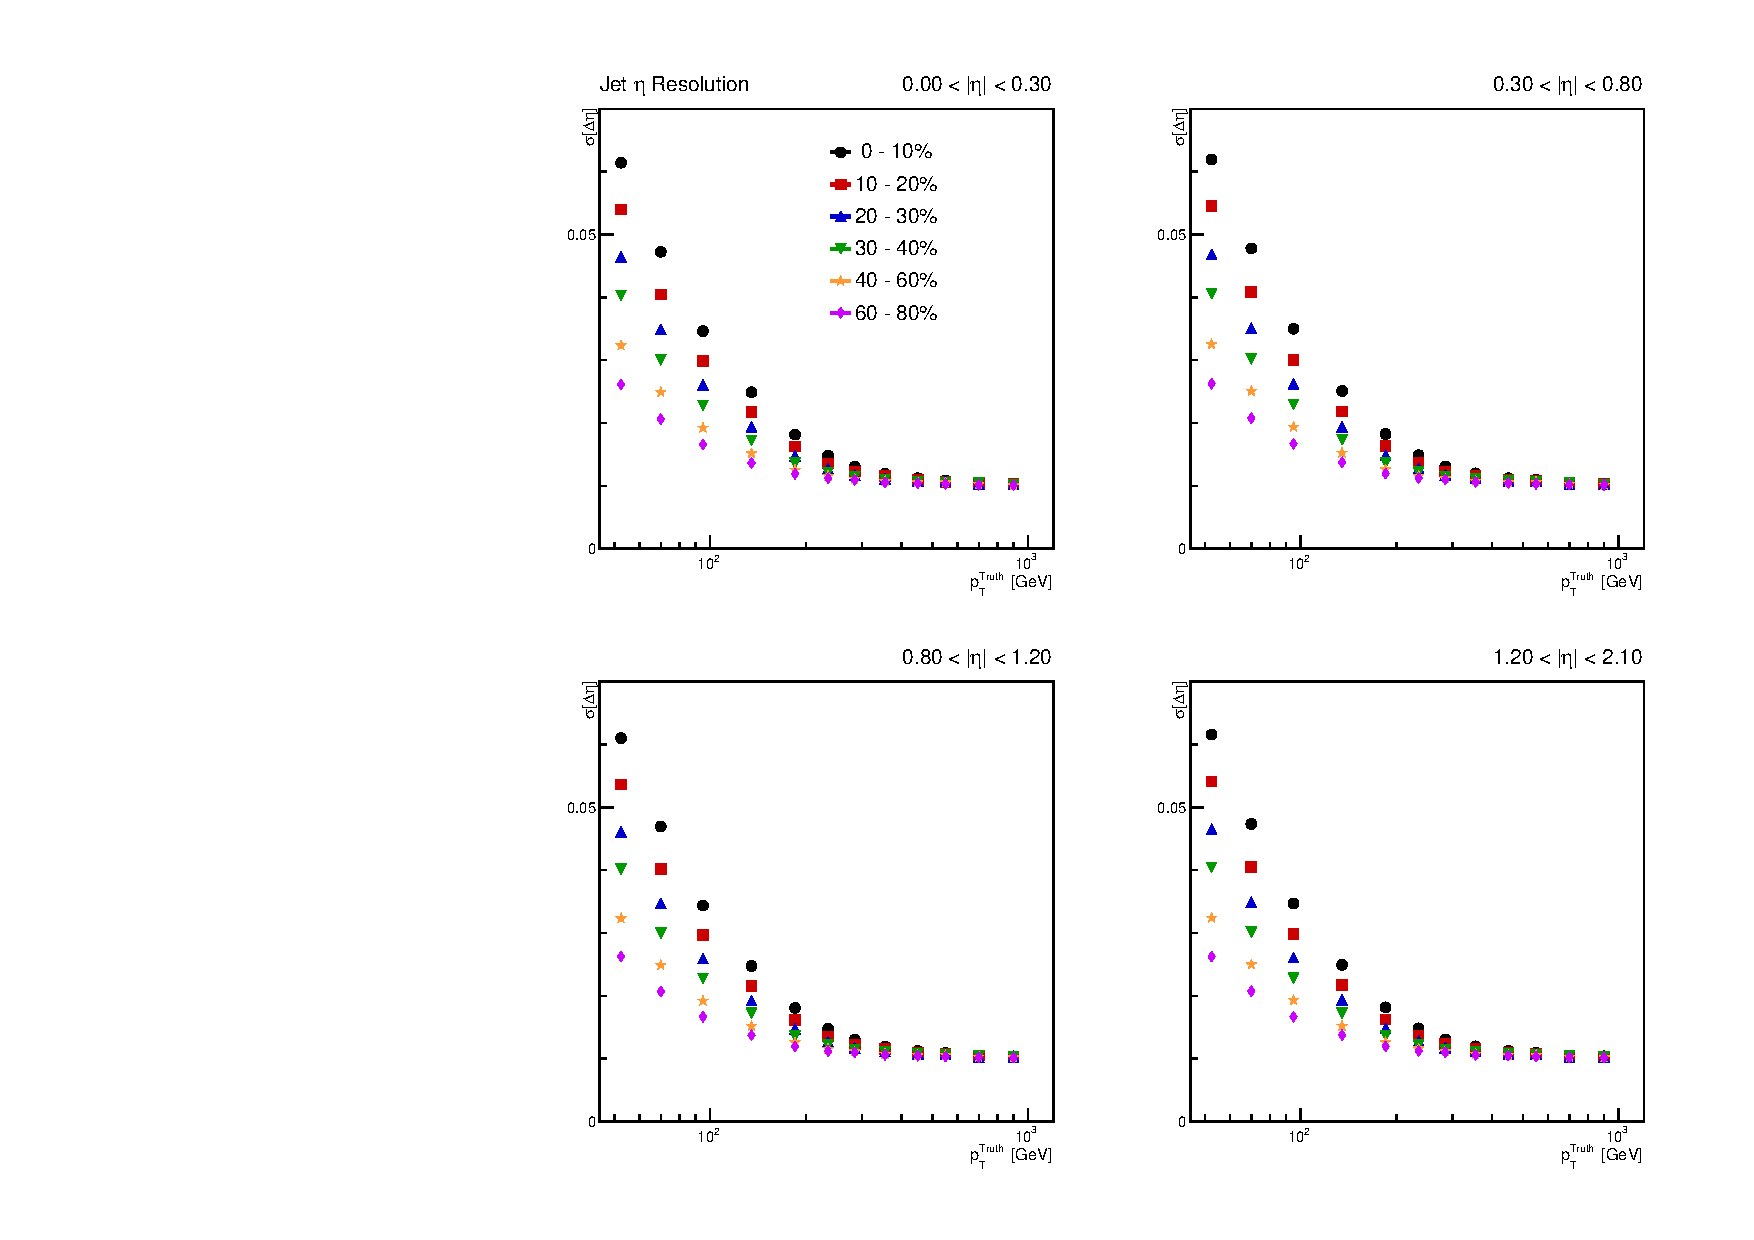
\includegraphics[width=\linewidth]{figures/setup/jet_res_eta_r04.pdf}}
          \caption{}
          \label{fig:nch_fcal}
\end{subfigure}
\qquad  \qquad  
\begin{subfigure}{.45\textwidth}  
  \centering
  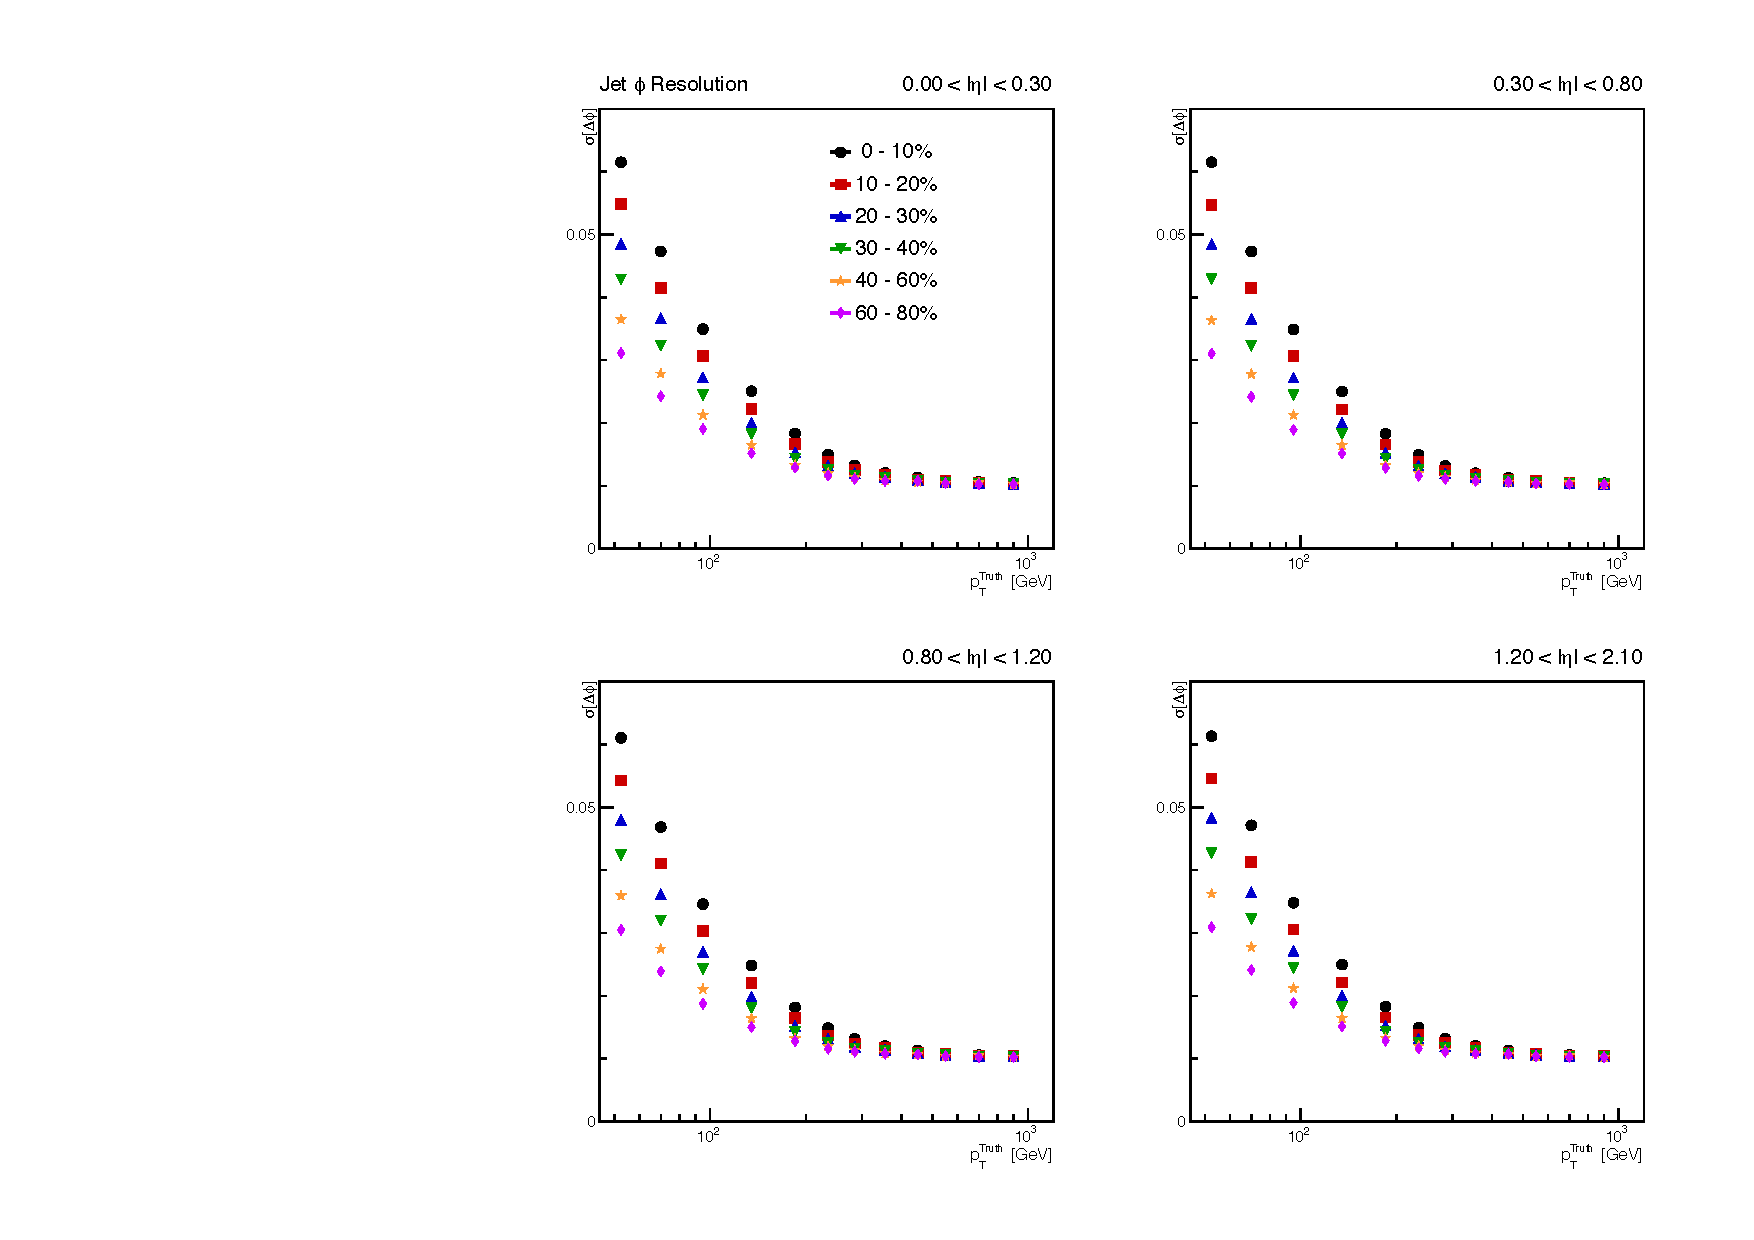
\includegraphics[width=\linewidth]{figures/setup/jet_res_phi_r04.pdf}}
          \caption{}
          \label{fig:fcal_distr}
\end{subfigure}
\caption{The (left) $\eta$ and (right) $\phi$ position resolution of the jet as a function of \pttruth\ in \pbpb\ collisions at $\sqrtsnn = 5.02$ TeV for different centrality and $\eta$ regions.
Figure taken from Ref.~\cite{Puri:2304504}.}
\label{fig:jet_posResolution}
\end{figure}




%The final corrections come from data driven (\insitu) methods like \pt\ balance studies (comparing the \pt\ of a jet and any other object like another jet, Z, or $\gamma$). Heavy ion collisions however, have the limitation that simple \pt\ balance studies are non-trivial because of jet quenching effects. Another limitation is the lack of high statistics for reference objects like $Z$'s and photons. The way to get around this is to derive a \textit{cross}-calibration, based on comparing jets in \pp\ collisions, as reconstructed by the heavy ion and \pp\ jet reconstruction algorithms. The HI jets can then be scaled with factors given by the ratio of $\langle \pt ^\hi / \pt^\emt \rangle$ in data and MC.
%
%The statistical uncertainties on the cross calibration factors come from the fits to the ratio of the relative response in data and MC, whereas the systematics come from changing the parameters of the study (these were evaluated as the maximum absolute difference between the nominal fit and any other iteration). The cross calibration factors for $0.8 < |\eta| < 1.2$, along with their uncertainties are shown on Fig.~\ref{fig:factors_w_uncertainties}. These are at the level of about 1\% and do not show strong variation with \pt. 
%\begin{figure}[htbp!]
%	\centering
%	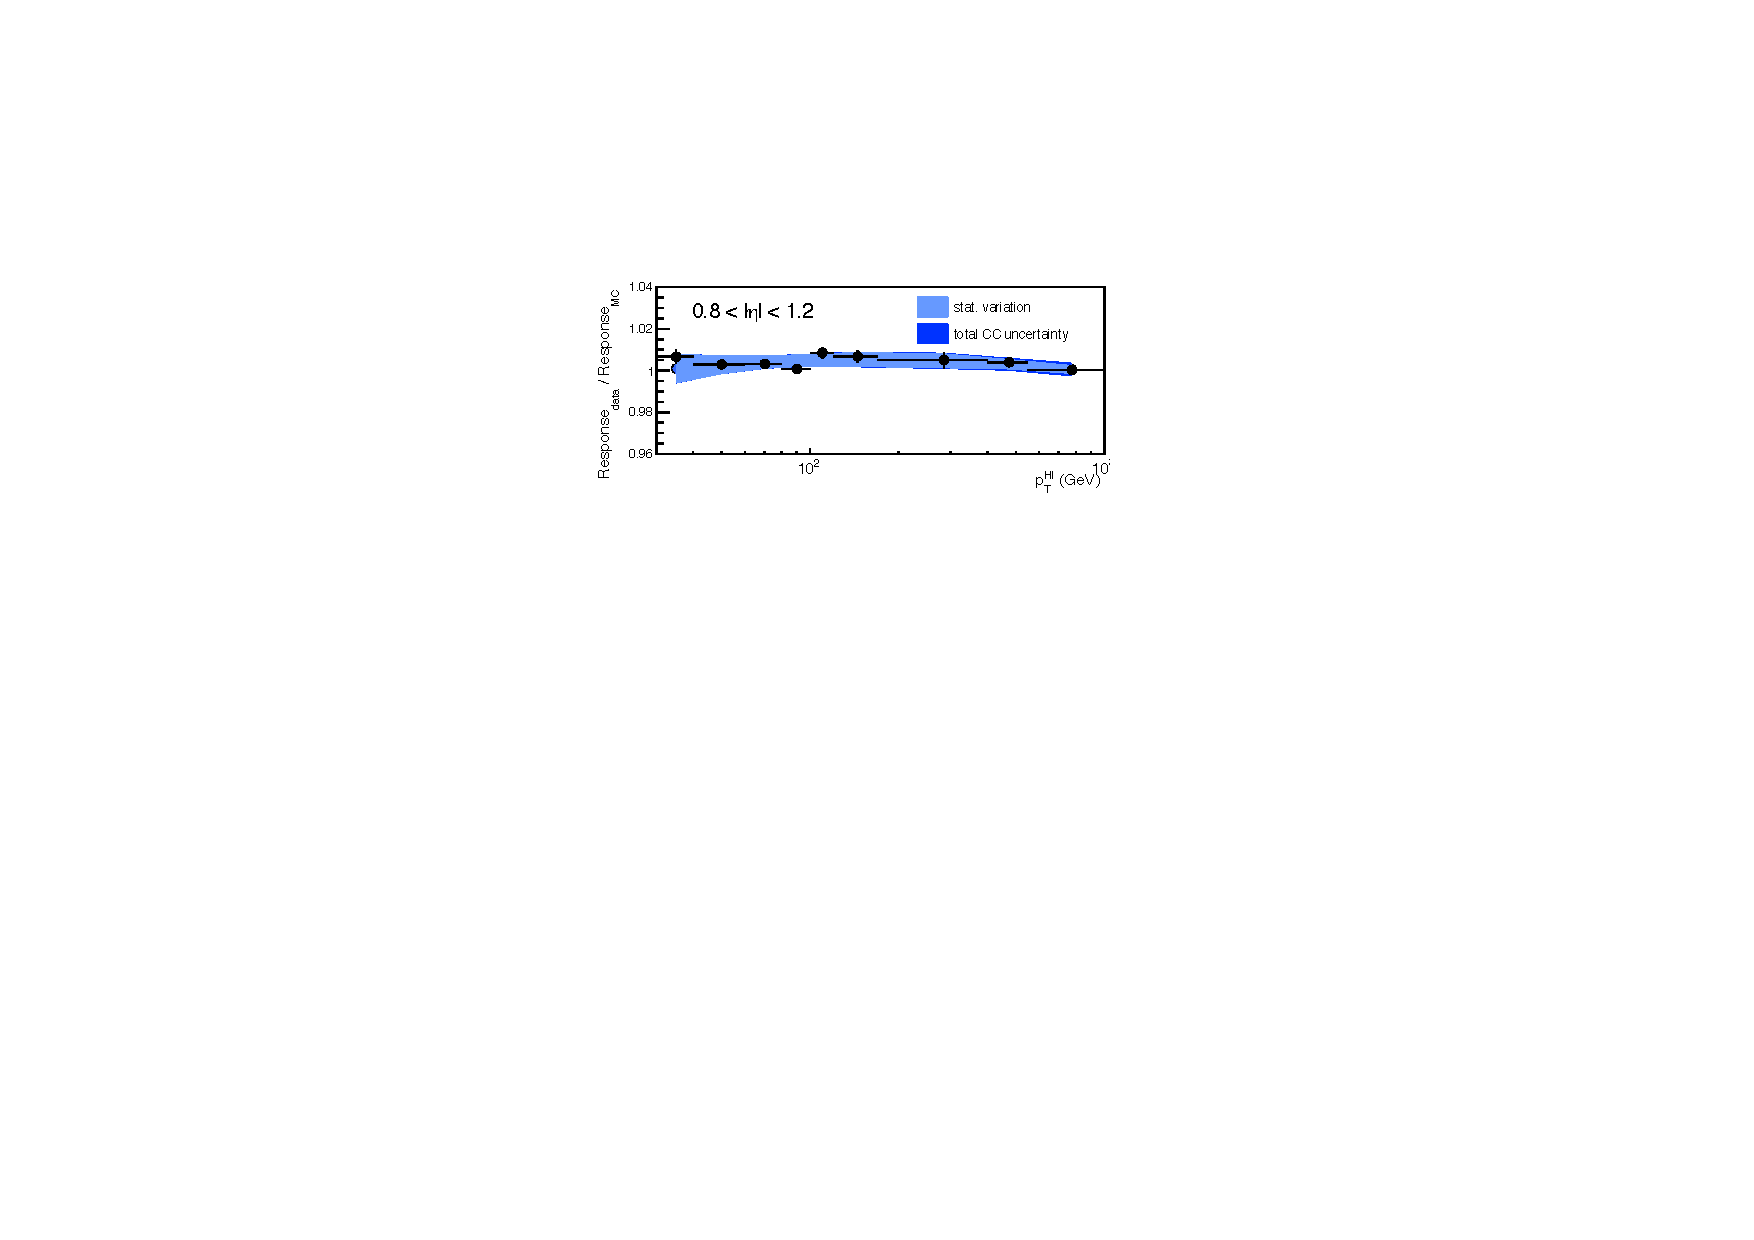
\includegraphics[width=0.5\textwidth]{figures/factors_w_uncertainties_2}
%	\caption{The cross calibration factors for $0.8 < |\eta| < 1.2$, as a function of $\textit{p}_{\text{T}}^{\text{HI}}$, along with their uncertainties.}
%	\label{fig:factors_w_uncertainties}%
%\end{figure}
%
%
%The cross-calibration procedure further allows applying the baseline jet energy scale/resolution uncertainties from the EMTopo jets, to the HI jets (along with the uncertainties of the cross-calibration procedure itself) \cite{xcalib_run1}. 
%
%
%\subsection{Heavy Ion Jet Energy Resolution Uncertainties}
%The uncertainty on the heavy ion jet energy resolution can be shown to be given by:
%
%\begin{equation}
%\delta \sigma_{\text{HI}} = \delta \sigma_{\text{EMTopo}} \sqrt{\left(1 + \frac{A}{\sigma_{\text{HI}}^2}\right)\left(1 + \left[\frac{\delta A}{2 \sigma_{\text{EMTopo}} \delta \sigma_{\text{EMTopo}}}\right)\right]^2} 
%\end{equation}
%where $\delta A ^2 = (2 s _{\text{HI}} \delta s _{\text{HI}})^2  + (2 s _{\text{EMTopo}} \delta s _{\text{EMTopo}})^2$ and $s^2_{\text{EMTopo/HI}}$ is the uncorrelated component between the errors in the jet \pt\, as reconstructed by two different algorithms applied to the same data \cite{xcalib_run1}. This result however, neglects that the uncertainty in the EMTopo jet energy resolution can be correlated with the systematic uncertainty on $A$. Accounting for this correlation, it can be shown that the uncertainty on the heavy ion jet energy resolution can be given by:
%\begin{equation}
%\dsigma_{{\text{HI}}} = \frac{\delta R_{{\text{HI}}}}{2 \sigma_{{\text{HI}}}}
%\end{equation}
%where
%\begin{align}
%R_{\text{HI}} &= \sigma_{\text{HI}}^2 \\
%\delta^2 R_{\text{HI}} &= \lambda^4 \delta^2 R_\emt + \delta^2 B \\
%\delta R_\emt  &= 2 \sigma_\emt \dsigma_\emt
%\end{align}
%Here, $\lambda$ accounts for the correlation between the HI and EMTopo jets, and $B$ is a estimate of the difference in the relative resolution between HI and EMTopo jets, as measured in data and MC.
%
%A comparison between $\delta\sigma_\emt$ and $\delta\sigma_{\text{HI}}$ can be seen in Fig.~\ref{fig:hi_jer_uncert}.
%
%
%\begin{figure}[htbp!]
%	\centering
%	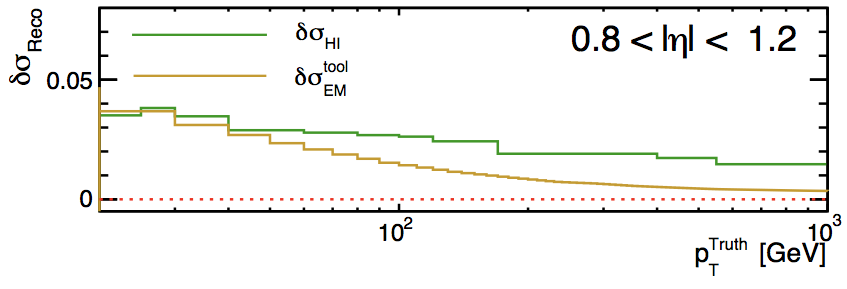
\includegraphics[width=0.7\textwidth]{uncert_2} %
%	\caption{The comparison between $\delta\sigma_\emt$ and $\delta\sigma_{\text{HI}}$ for $0.8 < |\eta| < 1.2$.}	
%	\label{fig:hi_jer_uncert}%
%\end{figure}
%


